%%%%%%%%%%%%%%%%%%%%%%%%%%%%%%%%%%%%%%%%%
% Classicthesis Typographic Thesis
% LaTeX Template
% Version 1.3 (15/2/14)
%
% This template has been downloaded from:
% http://www.LaTeXTemplates.com
%
% Original author:
% André Miede (http://www.miede.de)
%
% License:
% CC BY-NC-SA 3.0 (http://creativecommons.org/licenses/by-nc-sa/3.0/)
%
% General Tips:
% 1) Make sure to edit the classicthesis-config.file
% 2) New enumeration (A., B., C., etc in small caps): \begin{aenumerate} \end{aenumerate}
% 3) For margin notes: \marginpar or \graffito{}
% 4) Do not use bold fonts in this style, it is designed around them
% 5) Use tables as in the examples
% 6) See classicthesis-preamble.sty for useful commands
%
%%%%%%%%%%%%%%%%%%%%%%%%%%%%%%%%%%%%%%%%%

%----------------------------------------------------------------------------------------
%	PACKAGES AND OTHER DOCUMENT CONFIGURATIONS
%----------------------------------------------------------------------------------------

\documentclass[
		twoside,openright,titlepage,numbers=noenddot,headinclude,%1headlines,
                footinclude=true,cleardoublepage=empty,
                BCOR=5mm,paper=a4,fontsize=11pt, % Binding correction, paper type and font size
                ngerman,american, % Languages
                ]{scrreprt} 
                
% Includes the file which contains all the document configurations and packages - make sure to edit this file
%%%%%%%%%%%%%%%%%%%%%%%%%%%%%%%%%%%%%%%%%
% Thesis Configuration File
%
% The main lines to change in this file are in the DOCUMENT VARIABLES
% section, the rest of the file is for advanced configuration.
%
%%%%%%%%%%%%%%%%%%%%%%%%%%%%%%%%%%%%%%%%%

%----------------------------------------------------------------------------------------
%	DOCUMENT VARIABLES
%	Fill in the lines below to enter your information into the thesis template
%	Each of the commands can be cited anywhere in the thesis
%----------------------------------------------------------------------------------------

% Remove drafting to get rid of the '[ Date - classicthesis version 4.0 ]' text at the bottom of every page
\PassOptionsToPackage{eulerchapternumbers,listings,drafting, pdfspacing, subfig,beramono,eulermath,parts}{classicthesis}
% Available options: drafting parts nochapters linedheaders eulerchapternumbers beramono eulermath pdfspacing minionprospacing tocaligned dottedtoc manychapters listings floatperchapter subfig
% Adding 'dottedtoc' will make page numbers in the table of contents flushed right with dots leading to them

\newcommand{\myTitle}{Master Thesis\xspace}
\newcommand{\mySubtitle}{Creating a thin client based flood simulation tool based on open source software\xspace}
\newcommand{\myDegree}{Doktor-Ingenieur (Dr.-Ing.)\xspace}
\newcommand{\EmilName}{Emil M{\o}ller Rasmussen\xspace}
\newcommand{\GiannisName}{Giannis Angelidis\xspace}
\newcommand{\DavidName}{David Nagy\xspace}
\newcommand{\myProf}{Thomas Balstr{\o}m\xspace}
\newcommand{\myOtherProf}{Put name here\xspace}
\newcommand{\mySupervisor}{Thomas Balstrøm\xspace}
\newcommand{\myFaculty}{Surveying, Planning and Land Management\xspace}
\newcommand{\myDepartment}{Geoinformatics\xspace}
\newcommand{\myUni}{Aalborg University, Copenhagen\xspace}
\newcommand{\myLocation}{Copenhagen\xspace}
\newcommand{\myTime}{June 2015\xspace}
\newcommand{\myVersion}{version 1.0\xspace}

%----------------------------------------------------------------------------------------
%	USEFUL COMMANDS
%----------------------------------------------------------------------------------------

\newcommand{\ie}{i.\,e.}
\newcommand{\Ie}{I.\,e.}
\newcommand{\eg}{e.\,g.}
\newcommand{\Eg}{E.\,g.} 

\newcounter{dummy} % Necessary for correct hyperlinks (to index, bib, etc.)
\providecommand{\mLyX}{L\kern-.1667em\lower.25em\hbox{Y}\kern-.125emX\@}

%----------------------------------------------------------------------------------------
%	PACKAGES
%----------------------------------------------------------------------------------------

\usepackage{lipsum} % Used for inserting dummy 'Lorem ipsum' text into the template

%------------------------------------------------

%-------------------------------

\usepackage{pgfgantt}

%-------------------------------
 
\PassOptionsToPackage{latin9}{inputenc} % latin9 (ISO-8859-9) = latin1+"Euro sign"
\usepackage{inputenc}
 
 %------------------------------------------------

%\PassOptionsToPackage{ngerman,american}{babel}  % Change this to your language(s)
% Spanish languages need extra options in order to work with this template
%\PassOptionsToPackage{spanish,es-lcroman}{babel}
\usepackage{babel}

%------------------------------------------------			

\PassOptionsToPackage{square,numbers}{natbib}
 \usepackage{natbib}
 
 %------------------------------------------------

\PassOptionsToPackage{fleqn}{amsmath} % Math environments and more by the AMS 
 \usepackage{amsmath}
 
 %------------------------------------------------

\PassOptionsToPackage{T1}{fontenc} % T2A for cyrillics
\usepackage{fontenc}

%------------------------------------------------

\usepackage{xspace} % To get the spacing after macros right

%------------------------------------------------

\usepackage{mparhack} % To get marginpar right

%------------------------------------------------

\usepackage{fixltx2e} % Fixes some LaTeX stuff 

%------------------------------------------------

\PassOptionsToPackage{smaller}{acronym} % Include printonlyused in the first bracket to only show acronyms used in the text
\usepackage{acronym} % nice macros for handling all acronyms in the thesis

%------------------------------------------------

%\renewcommand*{\acsfont}[1]{\textssc{#1}} % For MinionPro
\renewcommand{\bflabel}[1]{{#1}\hfill} % Fix the list of acronyms

%------------------------------------------------

\PassOptionsToPackage{pdftex}{graphicx}
\usepackage{graphicx} 

%----------------------------------------------------------------------------------------
%	FLOATS: TABLES, FIGURES AND CAPTIONS SETUP
%----------------------------------------------------------------------------------------

\usepackage{tabularx} % Better tables
\setlength{\extrarowheight}{3pt} % Increase table row height
\newcommand{\tableheadline}[1]{\multicolumn{1}{c}{\spacedlowsmallcaps{#1}}}
\newcommand{\myfloatalign}{\centering} % To be used with each float for alignment
\usepackage{caption}
\captionsetup{format=hang,font=small}
\usepackage{subfig}  

%----------------------------------------------------------------------------------------
%	CODE LISTINGS SETUP
%----------------------------------------------------------------------------------------

\usepackage{listings} 
%\lstset{emph={trueIndex,root},emphstyle=\color{BlueViolet}}%\underbar} % for special keywords

\definecolor{keywords}{RGB}{255,0,90}
\definecolor{comments}{RGB}{0,0,113}
\definecolor{red}{RGB}{160,0,0}
\definecolor{green}{RGB}{0,150,0}
 
\lstset{language=Python, 
        basicstyle=\ttfamily\small, 
        keywordstyle=\color{keywords},
        commentstyle=\color{comments},
        stringstyle=\color{red},
        showstringspaces=false,
        identifierstyle=\color{green},
        procnamekeys={def,class},
        frame=single,
        stepnumber=5,
        breaklines=true}

%----------------------------------------------------------------------------------------
%	HYPERREFERENCES
%----------------------------------------------------------------------------------------

\PassOptionsToPackage{pdftex,hyperfootnotes=false,pdfpagelabels}{hyperref}
\usepackage{hyperref}  % backref linktocpage pagebackref
\pdfcompresslevel=9
\pdfadjustspacing=1

\hypersetup{
% Uncomment the line below to remove all links (to references, figures, tables, etc)
%draft, 
colorlinks=true, linktocpage=true, pdfstartpage=3, pdfstartview=FitV,
% Uncomment the line below if you want to have black links (e.g. for printing black and white)
%colorlinks=false, linktocpage=false, pdfborder={0 0 0}, pdfstartpage=3, pdfstartview=FitV, 
breaklinks=true, pdfpagemode=UseNone, pageanchor=true, pdfpagemode=UseOutlines,
plainpages=false, bookmarksnumbered, bookmarksopen=true, bookmarksopenlevel=1,
hypertexnames=true, pdfhighlight=/O, urlcolor=webbrown, linkcolor=RoyalBlue, citecolor=webgreen,
%------------------------------------------------
% PDF file meta-information
pdftitle={\myTitle},
pdfauthor={\textcopyright\ \myName, \myUni, \myFaculty},
pdfsubject={},
pdfkeywords={},
pdfcreator={pdfLaTeX},
pdfproducer={LaTeX with hyperref and classicthesis}
%------------------------------------------------
}   

%----------------------------------------------------------------------------------------
%	BACKREFERENCES
%----------------------------------------------------------------------------------------

\usepackage{ifthen} % Allows the user of the \ifthenelse command
\newboolean{enable-backrefs} % Variable to enable backrefs in the bibliography
\setboolean{enable-backrefs}{false} % Variable value: true or false

\newcommand{\backrefnotcitedstring}{\relax} % (Not cited.)
\newcommand{\backrefcitedsinglestring}[1]{(Cited on page~#1.)}
\newcommand{\backrefcitedmultistring}[1]{(Cited on pages~#1.)}
\ifthenelse{\boolean{enable-backrefs}} % If backrefs were enabled
{
\PassOptionsToPackage{hyperpageref}{backref}
\usepackage{backref} % to be loaded after hyperref package 
\renewcommand{\backreftwosep}{ and~} % separate 2 pages
\renewcommand{\backreflastsep}{, and~} % separate last of longer list
\renewcommand*{\backref}[1]{}  % disable standard
\renewcommand*{\backrefalt}[4]{% detailed backref
\ifcase #1 
\backrefnotcitedstring
\or
\backrefcitedsinglestring{#2}
\else
\backrefcitedmultistring{#2}
\fi}
}{\relax} 

%----------------------------------------------------------------------------------------
%	AUTOREFERENCES SETUP
%	Redefines how references in text are prefaced for different 
%	languages (e.g. "Section 1.2" or "section 1.2")
%----------------------------------------------------------------------------------------

\makeatletter
\@ifpackageloaded{babel}
{
\addto\extrasamerican{
\renewcommand*{\figureautorefname}{Figure}
\renewcommand*{\tableautorefname}{Table}
\renewcommand*{\partautorefname}{Part}
\renewcommand*{\chapterautorefname}{Chapter}
\renewcommand*{\sectionautorefname}{Section}
\renewcommand*{\subsectionautorefname}{Section}
\renewcommand*{\subsubsectionautorefname}{Section}
}
\addto\extrasngerman{
\renewcommand*{\paragraphautorefname}{Absatz}
\renewcommand*{\subparagraphautorefname}{Unterabsatz}
\renewcommand*{\footnoteautorefname}{Fu\"snote}
\renewcommand*{\FancyVerbLineautorefname}{Zeile}
\renewcommand*{\theoremautorefname}{Theorem}
\renewcommand*{\appendixautorefname}{Anhang}
\renewcommand*{\equationautorefname}{Gleichung}
\renewcommand*{\itemautorefname}{Punkt}
}
\providecommand{\subfigureautorefname}{\figureautorefname} % Fix to getting autorefs for subfigures right
}{\relax}
\makeatother

%----------------------------------------------------------------------------------------

\usepackage{classicthesis} 

%----------------------------------------------------------------------------------------
%	CHANGING TEXT AREA 
%----------------------------------------------------------------------------------------

%\linespread{1.05} % a bit more for Palatino
%\areaset[current]{312pt}{761pt} % 686 (factor 2.2) + 33 head + 42 head \the\footskip
%\setlength{\marginparwidth}{7em}%
%\setlength{\marginparsep}{2em}%

%----------------------------------------------------------------------------------------
%	USING DIFFERENT FONTS
%----------------------------------------------------------------------------------------

%\usepackage[oldstylenums]{kpfonts} % oldstyle notextcomp
%\usepackage[osf]{libertine}
%\usepackage{hfoldsty} % Computer Modern with osf
%\usepackage[light,condensed,math]{iwona}
%\renewcommand{\sfdefault}{iwona}
%\usepackage{lmodern} % <-- no osf support :-(
%\usepackage[urw-garamond]{mathdesign} <-- no osf support :-(

\begin{document}

\frenchspacing % Reduces space after periods to make text more compact

\raggedbottom % Makes all pages the height of the text on that page

\selectlanguage{american} % Select your default language - e.g. american or ngerman

%\renewcommand*{\bibname}{new name} % Uncomment to change the name of the bibliography
%\setbibpreamble{} % Uncomment to include a preamble to the bibliography - some text before the reference list starts

\pagenumbering{roman} % Roman page numbering prior to the start of the thesis content (i, ii, iii, etc)

\pagestyle{plain} % Suppress headers for the pre-content pages

%----------------------------------------------------------------------------------------
%	PRE-CONTENT THESIS PAGES
%----------------------------------------------------------------------------------------

% Title Page

\begin{titlepage}

\begin{addmargin}[-1cm]{-3cm}
\begin{center}
\large

\hfill
\vfill

\begingroup
\color{Maroon}\spacedallcaps{\myTitle} \\ \bigskip % Thesis title
\endgroup

\spacedlowsmallcaps{\myName} % Your name

\vfill


\includegraphics[width=6cm]{gfx/TFZsuperellipse_bw} \\ \medskip % Picture

\mySubtitle \\ \medskip % Thesis subtitle
%\myDegree \\
%\myDepartment \\
%\myFaculty \\
%\myUni \\ \bigskip

\myTime\ -- \myVersion % Time and version

\vfill

\end{center}
\end{addmargin}

\end{titlepage} % Main title page

% Back of the title page

\thispagestyle{empty}

\hfill

\vfill

%\noindent\myName: \textit{\myTitle,} \mySubtitle, %\myDegree, 
%\textcopyright\ \myTime

% You may wish to do something with the back of the title page, such as including your supervisors, location or time frame of the work. Below is an example of doing so although you may want to tweak it to your liking.

%\bigskip

%\noindent\spacedlowsmallcaps{Supervisors}: \\
%\myProf \\
%\myOtherProf \\ 
%\mySupervisor

%\medskip \\

%\noindent\spacedlowsmallcaps{Location}: \\
%\myLocation

%\medskip \\

%\noindent\spacedlowsmallcaps{Time Frame}: \\
%\myTime
 % Back of the title page

%\cleardoublepage\include{FrontBackMatter/Foreword} % Uncomment and create a Foreword.tex to include a foreword

\cleardoublepage% Abstract

\pdfbookmark[1]{Abstract}{Abstract} % Bookmark name visible in a PDF viewer

\begingroup
\let\clearpage\relax
\let\cleardoublepage\relax
\let\cleardoublepage\relax

\chapter*{Abstract} % Abstract name

Short summary of the contents\dots

\endgroup			

\vfill % Abstract page
\cleardoublepage% Acknowledgements

\pdfbookmark[1]{Acknowledgements}{Acknowledgements} % Bookmark name visible in a PDF viewer

\begin{flushright}{\slshape    
We have seen that computer programming is an art, \\ 
because it applies accumulated knowledge to the world, \\ 
because it requires skill and ingenuity, and especially \\
because it produces objects of beauty.} \\ \medskip
--- \defcitealias{knuth:1974}{Donald E. Knuth}\citetalias{knuth:1974} \citep{knuth:1974}
\end{flushright}

\bigskip

%----------------------------------------------------------------------------------------

\begingroup

\let\clearpage\relax
\let\cleardoublepage\relax
\let\cleardoublepage\relax

\chapter*{Acknowledgements} % Acknowledgements section text

\noindent A big thanks goes out to Thomas Balstrøm for his supervision during the creation of this process.
Thank you to the Open Source community, who made this project possible

\bigskip

\endgroup % Acknowledgements page

\pagestyle{scrheadings} % Show chapter titles as headings

\cleardoublepage% Table of Contents - List of Tables/Figures/Listings and Acronyms

\refstepcounter{dummy}

\pdfbookmark[1]{\contentsname}{tableofcontents} % Bookmark name visible in a PDF viewer

\setcounter{tocdepth}{2} % Depth of sections to include in the table of contents - currently up to subsections

\setcounter{secnumdepth}{3} % Depth of sections to number in the text itself - currently up to subsubsections

\manualmark
\markboth{\spacedlowsmallcaps{\contentsname}}{\spacedlowsmallcaps{\contentsname}}
\tableofcontents 
\automark[section]{chapter}
\renewcommand{\chaptermark}[1]{\markboth{\spacedlowsmallcaps{#1}}{\spacedlowsmallcaps{#1}}}
\renewcommand{\sectionmark}[1]{\markright{\thesection\enspace\spacedlowsmallcaps{#1}}}

\clearpage

\begingroup 
\let\clearpage\relax
\let\cleardoublepage\relax
\let\cleardoublepage\relax

%----------------------------------------------------------------------------------------
%	List of Figures
%----------------------------------------------------------------------------------------

\refstepcounter{dummy}
%\addcontentsline{toc}{chapter}{\listfigurename} % Uncomment if you would like the list of figures to appear in the table of contents
\pdfbookmark[1]{\listfigurename}{lof} % Bookmark name visible in a PDF viewer

\listoffigures

\vspace*{8ex}
\newpage

%----------------------------------------------------------------------------------------
%	List of Tables
%----------------------------------------------------------------------------------------

\refstepcounter{dummy}
%\addcontentsline{toc}{chapter}{\listtablename} % Uncomment if you would like the list of tables to appear in the table of contents
\pdfbookmark[1]{\listtablename}{lot} % Bookmark name visible in a PDF viewer

\listoftables
        
\vspace*{8ex}

                   
\endgroup % Contents, list of figures/tables/listings and acronyms

\cleardoublepage

\pagenumbering{arabic} % Arabic page numbering for thesis content (1, 2, 3, etc)
%\setcounter{page}{90} % Uncomment to manually start the page counter at an arbitrary value (for example if you wish to count the pre-content pages in the page count)

\cleardoublepage % Avoids problems with pdfbookmark

%----------------------------------------------------------------------------------------
%	THESIS CONTENT - CHAPTERS
%----------------------------------------------------------------------------------------


% Chapter 1

\chapter{Introduction \& problem statement} % Chapter title

\label{ch:introduction} % For referencing the chapter elsewhere, use \autoref{ch:introduction} 

%----------------------------------------------------------------------------------------

Here will be the introduction when it is finished. It will take up some room and be really awesome. % \citep{bringhurst:2002}.

\paragraph{Important Note:} During the last decade, GIS has undergone an incredible evolution, and open source software is becoming more widespread within a wide variety of sectors.

As the software develops, it no longer needs special skills to use it. 

Hydrological modelling. 

Hydrological modelling has always been a staple of GIScan be 

Flooding is one of the sectors that could use this
\noindent Therefore, please do not break the beauty of the style by changing these things unless you really know what you are doing! Please.

%----------------------------------------------------------------------------------------

\section{Problem statement}
A very important factor for successful thesis writing is the organization of the material. This template suggests a structure as the following:
\begin{itemize}
\item Creation of a thin client based flood simulation and management tool using open source technologies
\end{itemize}

\noindent This problem should enable us to do a ton of work in absolutely no time, motherfucker!.

%----------------------------------------------------------------------------------------

\section{Style Options}\label{sec:options}

There are a couple of options for \texttt{classicthesis.sty} that allow for a bit of freedom concerning the layout: \marginpar{\dots or your supervisor might use the margins for some comments of her own while reading.}
\begin{itemize}
\item General:
\begin{itemize}
\item\texttt{drafting}: prints the date and time at the bottom of each page, so you always know which version you are dealing with. Might come in handy not to give your Prof. that old draft.
\end{itemize}
	
\item Parts and Chapters:
\begin{itemize}
\item\texttt{parts}: if you use Part divisions for your document, you should choose this option. (Cannot be used together with \texttt{nochapters}.)

\item\texttt{nochapters}: allows to use the look-and-feel with classes that do not use chapters, \eg, for articles. Automatically turns off a couple of other options: \texttt{eulerchapternumbers}, \texttt{linedheaders}, \texttt{listsseparated}, and \texttt{parts}. 

\item\texttt{linedheaders}: changes the look of the chapter headings a bit by adding a horizontal line above the chapter title. The chapter number will also be moved to the top of the page, above the chapter title.
\end{itemize}

\item Typography:
\begin{itemize}
\item\texttt{eulerchapternumbers}: use figures from Hermann Zapf's Euler math font for the chapter numbers. By default, old style figures from the Palatino font are used.

\item\texttt{beramono}: loads Bera Mono as typewriter font. (Default setting is using the standard CM typewriter font.)
\item\texttt{eulermath}: loads the awesome Euler fonts for math. (Palatino is used as default font.)

\item\texttt{pdfspacing}: makes use of pdftex' letter spacing capabilities via the \texttt{microtype} package.\footnote{Use \texttt{microtype}'s \texttt{DVIoutput} option to generate DVI with pdftex.} This fixes some serious issues regarding math formul\ae\ etc. (\eg, ``\ss'') in headers. 

\item\texttt{minionprospacing}: uses the internal \texttt{textssc} command of the \texttt{MinionPro} package for letter spacing. This automatically enables the \texttt{minionpro} option and overrides the \texttt{pdfspacing} option.
\end{itemize}  

\item Table of Contents:
\begin{itemize}
\item\texttt{tocaligned}: aligns the whole table of contents on the left side. Some people like that, some don't.

\item\texttt{dottedtoc}: sets pagenumbers flushed right in the table of contents.

\item\texttt{manychapters}: if you need more than nine chapters for your document, you might not be happy with the spacing between the chapter number and the chapter title in the Table of Contents. This option allows for additional space in this context. However, it does not look as ``perfect'' if you use \verb|\parts| for structuring your document.
\end{itemize}

\item Floats:
\begin{itemize}
\item\texttt{listings}: loads the \texttt{listings} package (if not already done) and configures the List of Listings accordingly.
    
\item\texttt{floatperchapter}: activates numbering per chapter for all floats such as figures, tables, and listings (if used).	
    
\item\texttt{subfig}(\texttt{ure}): is passed to the \texttt{tocloft} package to enable compatibility with the \texttt{subfig}(\texttt{ure}) package. Use this option if you want use classicthesis with the \texttt{subfig} package.

\end{itemize}    

\end{itemize}

\noindent The best way to figure these options out is to try the different possibilities and see, what you and your supervisor like best.

In order to make things easier in general, \texttt{classicthesis-config.tex} contains some useful commands that might help you.

%----------------------------------------------------------------------------------------

\section{Customization}\label{sec:custom}

This section will give you some hints about how to adapt \texttt{classicthesis} to your needs.

The file \texttt{classicthesis.sty} contains the core functionality of the style and in most cases will be left intact, whereas the file \texttt{classic\-thesis-config.tex} is used for some common user customizations. 

The first customization you are about to make is to alter the document title, author name, and other thesis details. In order to do this, replace the data in the following lines of \texttt{classicthesis-config.tex:}\marginpar{Modifications in \texttt{classic\-thesis-config.tex}
}

\begin{lstlisting}[frame=lt]
\newcommand{\myTitle}{A Classic Thesis Style\xspace}
\newcommand{\mySubtitle}{An Homage to ...\xspace}
\newcommand{\myDegree}{Doktor-Ingenieur (Dr.-Ing.)\xspace}
\end{lstlisting}

Further customization can be made in \texttt{classicthesis-config.tex} by choosing the options to \texttt{classicthesis.sty} (see~\autoref{sec:options}) in a line that looks like this:

\begin{lstlisting}[frame=lt]
\PassOptionsToPackage{eulerchapternumbers,listings,drafting, pdfspacing, subfig,beramono,eulermath,parts}{classicthesis}

\end{lstlisting}

If you want to use backreferences from your citations to the pages they were cited on, change the following line from:
\begin{lstlisting}[breaklines=false,frame=lt]
\setboolean{enable-backrefs}{false}
\end{lstlisting}
to
\begin{lstlisting}[breaklines=false,frame=lt]
\setboolean{enable-backrefs}{true}
\end{lstlisting}

Many other customizations in \texttt{classicthesis-config.tex} are possible, but you should be careful making changes there, since some changes could cause errors.

Finally, changes can be made in the file \texttt{classicthesis.sty}, \marginpar{Modifications in \texttt{classicthesis.sty}} although this is mostly not designed for user customization. The main change that might be made here is the text-block size, for example, to get longer lines of text.

%----------------------------------------------------------------------------------------

\section{Issues}\label{sec:issues}
This section will list some information about problems using \texttt{classic\-thesis} in general or using it with other packages.

Beta versions of \texttt{classicthesis} can be found at the following Google code repository:
\begin{center}
\url{http://code.google.com/p/classicthesis/}
\end{center}

\noindent There, you can also post serious bugs and problems you encounter.

\subsection*{Compatibility with the \texttt{glossaries} Package}
If you want to use the \texttt{glossaries} package, take care of loading it with the following options:
\begin{verbatim}
\usepackage[style=long,nolist]{glossaries}
\end{verbatim}

\noindent Thanks to Sven Staehs for this information. 

\subsection*{Compatibility with the (Spanish) \texttt{babel} Package}
Spanish languages need an extra option in order to work with this template:
\begin{verbatim}
\usepackage[spanish,es-lcroman]{babel}
\end{verbatim}

\noindent Thanks to an unknown person for this information (via Google Code issue reporting). 

\subsection*{Compatibility with the \texttt{pdfsync} Package}
Using the \texttt{pdfsync} package leads to linebreaking problems with the \texttt{graffito} command. Thanks to Henrik Schumacher for this information. 

%----------------------------------------------------------------------------------------

\section{Future Work}
So far, this is a quite stable version that served a couple of people well during their thesis time. However, some things are still not as they should be. Proper documentation in the standard format is still missing. In the long run, the style should probably be published separately, with the template bundle being only an application of the style. Alas, there is no time for that at the moment\dots it could be a nice task for a small group of \LaTeX nicians.

Please do not send me email with questions concerning \LaTeX\ or the template, as I do not have time for an answer. But if you have comments, suggestions, or improvements for the style or the template in general, do not hesitate to write them on that postcard of yours.

%----------------------------------------------------------------------------------------

\section{License}
\paragraph{GNU General Public License:} This program is free software; you can redistribute it and/or modify it under the terms of the \textsmaller{GNU} General Public License as published by the Free Software Foundation; either version 2 of the License, or (at your option) any later version.

This program is distributed in the hope that it will be useful, but \emph{without any warranty}; without even the implied warranty of \emph{merchantability} or \emph{fitness for a particular purpose}. See the \textsmaller{GNU} General Public License for more details. % Chapter 1
% Chapter 1

\chapter{Theory} % Chapter title

\label{ch:theory} % For referencing the chapter elsewhere, use \autoref{ch:introduction} 

%----------------------------------------------------------------------------------------

\section{GRASS}

GRASS (Geographical Resources Analysis Support System) is an open source GIS desktop application capable of handling spatial data in both vector and raster formats. 
GRASS adopted a GNU GPL \footnote{General Public License, see http://www.gnu.org} in 1999, which allowed users and developers to have free access to the GRASS source code, resulting in a library of more than 350 freely available modules capable of management, processing, analysis and visualization of geospatial data \citep{GRASSGIS}.\\
Because Open Source GIS provides full access to its internal structure and algorithms, unlike proprietary GIS software, users can learn from existing modules and create their own GIS modules based on the preexisting ones. GRASS libraries can also be accessed through the built-in API (Application Programming Interface). This enables a more efficient integration of new functionalities into the GRASS environment – Most GIS applications can be written in the Python, making it possible to automate work-flows.
As mentioned earlier, GRASS contains around 350 modules, which can be accessed using GRASS' graphic interface. The three main module-groups are based on vector, raster, and imagery analysis \citep{grassbook}.\\

A grass project is located in GRASS' designated database folder \textit{grassdata}(also known as GRASS' GISBASE). This is the directory where processed or imported data is stored and, unless otherwise designated, where most of the processing will occur. 
A project in created in GRASS has to have both a \textsc{LOCATION} and a \textsc{MAPSET}.
The most important of these is the \textsc{LOCATION}. This is where the critical information about the project, such as the projection of the data, is stored. 
GRASS does not have reprojecting on-the-fly functionality – as ArcGIS or QGIS are capable of. Using the \textsc{LOCATION} folder properly is therefore necessary. 
The \textsc{MAPSET} is a way of separating different projects, or phases of processes, and a LOCATION can contain several \textsc{MAPSETS}\citep{grassbook}. 

GRASS can be operated by a variety of ways. The most commonly used method is by accessing the modules through the GRASS GUI (Graphical User Interface), but it can also be achieved purely through scripting – such as with Python. GRASS is able to handle most of the vector and raster formats which are supported by GDAL (Geospatial Data Abstraction Library), such as GeoTIFF, ArcGRID, ERDAS, USGS SDTS DEM, etc \citep{GRASSGIS}. \\

The way GRASS handles region and resolution settings differs from most other GIS software. Since different datasets can have different extents, it is possible to set the current processing region allowing the user to run a specific process on a subset of a raster or the location and not necessarily run a process on the entire image. 
The lack of on-the-fly reprojection makes GRASS less user-friendly than other similar products. Furthermore it does not allow drag and drop import, and most functions must be invoked using the built-in GRASS commandline-like utilities \citep{grassbook}.

\subsection{Hydrology in GIS}

The accurate depiction of hydrological movements and their responses to the land cover has been the objective of hydrological scientists for many decades. As advances in IT have progressed, the calculations and algorithms possible have become more sophisticated, accurate and faster. \\

When investigating hydrological conditions, DEM (Digital Elevation Models) are used. Because of this, the results are dependent on the quality of the model being used. Most major GIS software have some built-in hydrology tools, capable of being incorporated into various workflows. To give an example of the application of hydrology in GRASS, this section will include a description of some of the main hydrology tools from GRASS' libraries.

\subsubsection{Flow direction}
Flow direction is a core hydrology tool. Flow direction makes it possible to determine which direction water will flow, when moving through a DEM. The computational algorithm can be created in a wide variety of ways, for instance GRASS' “r.terraflow” module has two options: 

\begin{itemize}
\item Multiple Flow Direction (MFD) 
\end{itemize}
or 
\begin{itemize}
\item Single Flow Direction (SFD)
\end{itemize}
 
Both of these algorithms are based on a so-called Moore-Neighborhood. This neighborhood involves the eight cells surrounding a specific cell on a raster. The basis of the flow direction is that the water flows to a cell with a lower value then the current one, but it is in this regard that MFD and SFD differ from each other. As can be seen from \autoref{fig:flowdirect}, the SFD method assigns a single flow direction to the lowest downslope neighboring cell, whilst MFD assigns flow direction to all downslope neighboring cells \citep{grassbook}. \\

\begin{figure}[t]
\centering
	{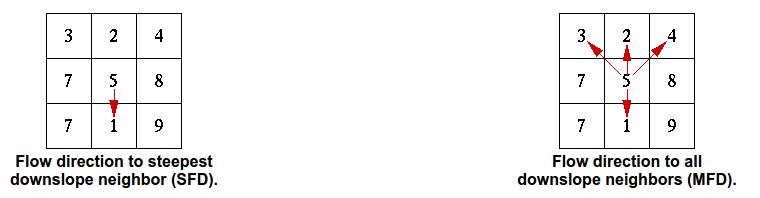
\includegraphics[width=\linewidth]{gfx/SFD_MFD.png}}
\caption{Example of two different flow direction methods \citep{sfdmfd}.}
\label{fig:flowdirect}
\end{figure}

Both methods have the criteria, that the flow direction cannot contribute to cells with the same height as the central cell or cells which have no downslope neighbors \citep{sfdmfd2}.
Pits or so called depressions or sinks, are areas which are surrounded by higher elevation values. It is also an internal drainage area, although some of the time it is a real natural feature such as a karst, but usually it is an imperfection of the digital elevation model.  The GRASS Terraflow module fills the sinks and then assign a Flow Direction on the filled terrain, thereby the flow direction will not be ruined by a DEM full of depressions \citep{sfdmfd}. 

\subsubsection{Flow accumulation}
Another important hydrology tool is Flow Accumulation. This tool is capable of calculating the flow running through the the terrain, such as the accumulation of water \citep{sfdmfd}. As input, the module needs a raster indicating flow directions. It should be noted that flow accumulation is highly dependent on the previous described phenomenas and computational methods. For example MFD would provide a significantly different flow accumulation than SFD, as MFD provides more accumulation possibilities. Also, a depressionless DEM will have a different accumulation than one with depressions \citep{sfdmfd}. Analyzing the direction of the flow can give a limited insight about cell behaviors, however flow accumulation allows the investigation of main stream lines, and how they contribute to the stream system, as well as providing the an output of stream lines.

\subsubsection{Watershed}
A Watershed is an area where all streams end up in a common outlet. This can also be called a basin or a catchment area, however in this paper it will be referred to as a watershed.\\


\begin{figure}[h]
\centering
	{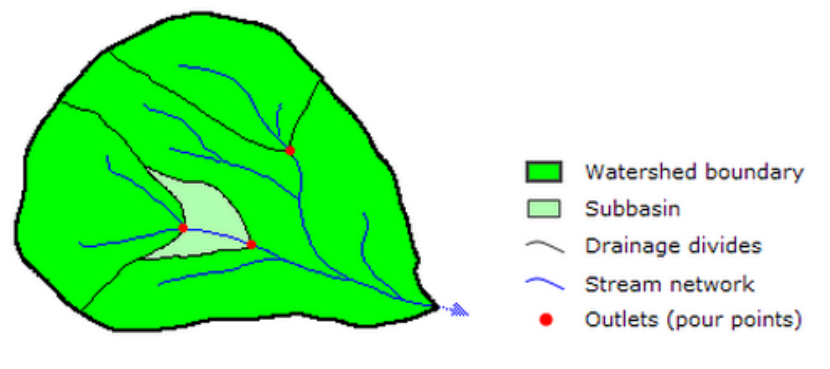
\includegraphics[width=\linewidth]{gfx/Watershed.png}}
\caption{Figure showing important concepts when working with watersheds \citep{watershed}.}
\end{figure}

A watershed is a relative term, as it depends on the scale at which you look at them – practically all streams have their own watershed. Therefore to determine the watersheds of a DEM, it is necessary to know a variety of factors, such as flow accumulation, flow direction or slope aspect of the terrain \citep{rwatershed}. \\
In  GRASS there is a watershed algorithm, which considers every aspect of the previously mentioned procedure. The watershed (r.watershed) module has watershed output which is created by the output of the flow direction and the derived flow accumulation output of the DEM. As mentioned earlier, watershed sizes are relative to the scale of the investigation. A threshold value can be set the to delineate the minimum size of the resultant watershed, based on the scale of interest \citep{grassbook} \citep{rwatershed}. Setting this value should be based on the horizontal resolution of the raster being worked on. For instance, setting the value to 1000 setup on a raster with 10mx10m resolution, would define, that the smallest watershed area has to be larger than 1000*10m*10m = 0,1km2.

\subsubsection{Cost Distance}
The Cost Distance analysis is used to calculate the route that will “cost” the least when traveling across a given surface \citep{grassbook}. This tool uses a cost surface to determine the weighted shortest path to the nearest source cells or source vector feature, and as such does not calculate distance in geographical units, but shows the distance by cost surface units \citep{rcost}. The cost can include several criteria, factors and weights depending on the specific analysis. For example, the cost surface of a hiking route can be established by taking into account the steepness, the type of the area or even the recommendations of which area should be visited.
Each of the factors chosen should be reclassified in order to put them on a common scale, so that they can be compared in spite of their different nature. 
The cost distance module of GRASS (r.cost) is based on the previously explained method \citep{rcost}. In order to get the cost distance output raster, the user needs to provide a cost raster.

\begin{figure}[t]
\centering
	{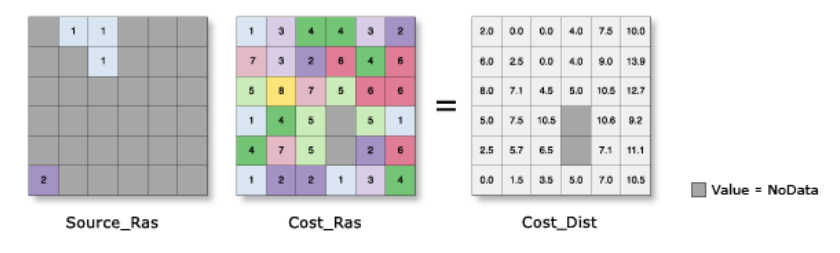
\includegraphics[width=\linewidth]{gfx/COST.png}}
\caption{Figure showing how cost distance works \citep{costdistance}.}
\end{figure}

%----------------------------------------------------------------------------------------

\section{Python}\label{sec:issues}

Python is a programming language used extensively within the geospatial world. A lot of GIS packages are either created with Python, or have built-in functionality to inferface with Python. The actual reason for this is generally not known, but it might be because Python is a language that \citep{pybook}:
\begin{itemize}
\item emphasizes code readability.
\item is compatible with all major operating systems, and usually comes pre-packaged with these. 
\item Is completely open source. 
\item is highly extensible. 
\end{itemize}
Being extensible, means that it does not come prepackaged with all functionality built in, but expects the user to download / add necessary libraries as they are needed. 
The most commonly used versions of Python are 2.7 and 3.x, which differ from each other for various reasons. The 2.7 release is a so-called legacy release, which means that it is not the worked-upon version, and wont see major updates. The 3.x is the newest version, and will be updated regularly. When working with “older” software, and libraries, it is most likely best to use version 2.7 as there will likely be compatibility issues when using a newer version of Python \citep{python}.\\

Standard python syntax looks something like this:\\

\begin{lstlisting}[language=Python]
import random
randomarray = [1,3,5,7,8]
for element in randomarray:
	print(element)
\end{lstlisting}

\section{GRASS}

From within GRASS, Python can easily be used to call native functionality. These functions can also be accessed and manipulated by using a variety of scripting languages, without explicitly starting the GRASS software. One of the languages capable of doing this is Python. \citep{grassbook} \\

Opening, and chaining, functions within GRASS can become tedious, and if wanting to run the same process a lot of times, it can be relevant to setup a workflow with a Python script.
The functions and modules of GRASS, when used outside of an actual GRASS session, only work when a series of specific environment variables have been set. 
These are \citep{grasswiki}:
\begin{itemize}
\item GISBASE needs to be set to the top-level directory of the GRASS installation. 
\item GISRC needs to contain the absolute path to a file containing settings for GISDBASE, LOCATION and MAPSET 
\item PATH needs to include \$GISBASE/bin and \$GISBASE/scripts.
\end{itemize}

An example of the syntax of GRASS functions being accessed externally through Python \citep{grasswiki}:

\begin{lstlisting}[language=Python]
import grass.script as gscript
import grass.script.setup as gsetup
gscript.run_command(“r.in.gdal”,flags=””,input=”input.tif”,output=”output”
\end{lstlisting}


\section{Web technologies}
\subsection{HTML}
In 1990, Tim Berners-Lee, a physicist employed at CERN, invented HTML by trying to organize the research documents available to scientists and facilitate their access to them. He is also considered by many the inventor of the Internet by having set the foundations of the web as we know it today \citep{htmlnet}.
HTML stands for HyperText Markup Language. To be more specific \citep{htmlnet},

\begin{itemize}
\item Hyper means that HTML does not perform commands in one line and then proceeds to the next one as Python or C++ does.
\item Text is self-explanatory
\item Markup means that the author can put tags in the text. This means that the text is structured in different sections such as the header, the body etc.
\item Language of course means that HTML is a programming language.
\end{itemize}

The following figure displays an example of a basic HTML code snippet. It will help in understanding the structure and content of an HTML document.

\begin{lstlisting}
<!DOCTYPE html>
<html>
<body>

<h1>My first heading!</h1>
<p>My first paragraph!</p>

</body>
</html>
\end{lstlisting}

Starting at the top, the DOCTYPE declaration, states what kind of document we are creating. In this case, we have an HTML document (w3shcools). In the html tags (<html>, </html>), we describe the page we are creating. The body tags (<body>, </body>) contains all the information visible to the user. Finally, the tags <h1> and <p>, set the heading and paragraphs respectively \citep{w3schools}.

\subsection{JavaScript}
JavaScript is a dynamic scripting language developed by Netscape. Brendan Eich, the original developer of JavaScript, created it so that it would be able to support prototype based object construction and  that it can work both as an object oriented and procedural language. Its syntax was developed to be similar to C++ and Java in order to minimize its learning curve \citep{mozjava}. Below, we can see a small example of JavaScript use in an HTML document.	

\begin{lstlisting}
<!DOCTYPE html>
<html>
<body>

<h1>My first JavaScript!	</h1>

<script>
document.write("<p>My First Javascript!</p>");
</script>

</body>
</html>
\end{lstlisting}

In this example, we have a basic HTML document and in the script tags (<script>, </script>) we can insert the JavaScript function that will be executed.

\section{PyWPS}

A Web Processing Service (WPS) is a standard defined by the Open Geospatial Consortium which describes how inputs and outputs (also called requests and responses) for geospatial processing services should be standardized. 
WPS Version 1.0 was released in June 2007, and WPS version version 2.0 was approved and released in January 2015 \citep{ogcwps}. \\
WPS defines how a client can request the a process is executed, and how the output is supposed to be handled. Furthermore, it defines the setup of the interface that enables publishing of geospatial processes, and the user's access to those processes. Through this implementation, it should become easier for people who want to publish custom geospatial functions on the internet, to do it in a similar and organized way. \\

One implementation of these standards is PyWPS. This service connects the web browser with a variety of tools installed on a server, such as GRASS GIS, GDAL, PROJ and R \citep{pywpsweb}. PyWPS does not process the data by it self but  it can work with GIS software such as GRASS, enabling the creation of GIS-based analytical web services, based on Python \citep{pywpsweb}. 
The WPS enables a user to Describe a Process, Execute a Process and to Get Capabilities of the server, and the instances available. Similar to other OGC Web Services (such as WMS, WFS or WCS), WPS has three basic request types. Namely GetCapabilities, DescribeProcess and Execute \citep{pywps}.\\

When requesting data from the server, the URL you send to the server, defines what kind of request you have made. Example strings for the three processes mentioned above:\\
\begin{itemize}
\item http://webaddress/pywps/?service=WPS&request=GetCapablities 
\item http://webaddress/pywps/?service=WPS&version=1.0.0&request=DescribeProcess&identifier=all
\item http://webaddress/pywps/?service=WPS&version=1.0.0&request=Execute&identifier=<PROCESS>&datainputs=[<INPUT1>=<VALUE>;<INPUT2>=<VALUE>]
\end{itemize}

When an Execute request has been posted to the WPS, it will start processing on the server, and when it is done outputs will be provided encoded in a standardized XML document. 
A PyWPS service must contain the following elements \citep{pywps}: 
\begin{itemize}
\item A class defining the initation of a WPS Process:
class Flooding(WPSProcess):
\item A function called \_\_init\_\_:
def \_\_init\_\_(self):
\item A function called execute:
def execute(self):
\end{itemize} \\

The init function contains a variety of settings relevant to the process being executed. Furthermore the inputs and outputs get defined, whilst the execute contains the code that is to be run. 
The PyWPS syntax for calling GRASS differs somewhat from when interfacing purely with Python. An example of GRASS accessed with PyWPS is:

\begin{lstlisting}[language=Python]
self.cmd(['r.in.gdal','input=%s' % self.rasterin.getValue(),'output=%s' % original,'-o'])
\end{lstlisting}

\section{Flask}

Flask is a web application framework written in Python. The framework is based on a so-called Web Server Gateway Interface (WSGI) called Werkzeug and a website templating engine called Jinja2. The framework is built to be as simple as possible, comes with a core of the most needed libraries, and expects further functionalities and modules to be imported as third-party libraries \citep{flaskbook}. \\
Several similar frameworks exist, but they either become very advanced, or very specialized. The Flask framework has a simple setup, and is easy to use. \citep{flaskbook} \\
By using Flask it is possible to quickly create a dynamic web environment, by writing it in a combination of Python and HTML. 
A simple application using Flask looks something like the following \citep{flaskweb}: 

\begin{lstlisting}[language=Python]
from flask import Flask
app = Flask(__name__)

@app.route("/")
def hello():
    return "Hello World!"

if __name__ == "__main__":
    app.run()
\end{lstlisting}

A website written in Flask consists of a variety of templates that change content depending on where on a site a user is, or wishes to visit. This is done by defining some general templates, and some blocks of content that get swapped out depending on the current view. 

%----------------------------------------------------------------------------------------

\section{Open Source GIS}

The definition of Open Source is clearly set by the Open Source Initiative (OSI), making it possible to clearly define define which licenses actually are "Open Source". In addition to this, the OSI provides certification to these licenses to indicate that they follow the open-source principles and comply with the Open Source definition. This definition states the following \citep{osbook}:
\begin{itemize}

\item The license should allow the sale or gifting of the software as a part of software distribution along with programs from several different sources. For such sale no royalty or monetary compensation should be required. ("The license shall not restrict any party from selling or giving away the software as a component of an aggregate software distribution containing programs from several different sources. The license shall not require a royalty or other fee for such sale".)
\item The source code of the software should be included in the software and it must be distributed freely along with the compiled form. In the case where the source code is not distributed with the software, an easily reached alternative must be provided, at most with a minimum reproduction cost.
\item Modifications and derived works must be allowed and distributes as freely as the software itself.
\item Modification of the source code can be restricted by the license only in the case that the license allows "patch files" distribution along with the source code for program modification. Software built from modified source code must be allowed to be distributed. \item Works derived from the source code may be required to have a different name or version number.
\item Discrimination against persons or groups is not allowed
\item All fields of endeavor must be allowed to use the software, unrestricted by its license.
In the case where the program is redistributed, the same rights must apply without the execution of an additional license from those parties.
\item In the case where the program is part of a specific software distribution, parties to whom the program is redistributed should have the same rights with those to  whom the original program is distributed.
\item Restrictions on other software, distributed with the licensed software must not be placed under restrictions.
\item Access to the license must not be dependable on any individual technology pr interface
\end{itemize}

\begin{figure}[h]
\centering
	{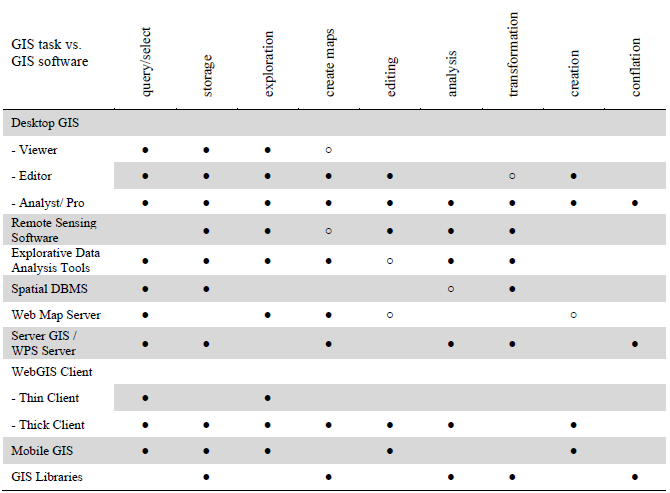
\includegraphics[width=\linewidth]{gfx/OS.png}}
\caption{Figure showing categorization of GIS software \citep{osarticle}}
\label{fig:giscategory}
\end{figure}

Some of the most common desktop GIS Software can be seen from \autoref{fig:giscategory}.
The main reason open software exists is because the US Government, during the 1970ies and 1980ies implemented changes in the patent laws that allowed software and hardware companies to unbundle software and hardware and the source code for software was under restricted access. For the reasons stated above the Free Software Foundation (FSF) was created \citep{osbookde}.


Due to their widespread need, Geographic Information Systems software are also available to the public under the "Open Source" label. These software include a wide variety of open source examples that can be divided based on the functionalities the offer. \autoref{tab:gissoftware} below can provide with some insight on such categorization.  


\begin{table}[h]
\caption{GIS software}
\begin{tabular}{l | r}
Desktop GIS Software & Developer \\ 
\hline
GRASS GIS & Neteler \& Mitasova, 2008; Neteler, Bowman, Landa \& Metz 2012 \\ 
\hline
QGIS & Hugentobler, 2008 \\ 
\hline
ILWIS / ILWIS Open & Valenzuela, 1988; Hengl, Gruber \& Shrestha, 2003 \\ 
\hline
uDig & Ramsey, 2006 \\ 
\hline
SAGA & Olaya 2004, Conrad 2007  \\ 
\hline
OpenJUMP & Steiniger \& Michaud, 2009 \\ 
\hline
MapWindow GIS & Ames, Michaelis \& Dunsford, 2007 \\ 
\hline
gvSIG & Anguix \& Diaz, 2008 \\ 
\hline
\end{tabular}
\caption*{Categorization of GIS software \citep{osarticle}.}
\label{tab:gissoftware}
\end{table}
% Chapter 1

\chapter{Methodology} % Chapter title

\label{ch:method} % For referencing the chapter elsewhere, use \autoref{ch:introduction} 

%----------------------------------------------------------------------------------------

The project startup was officially set to be the 2nd of February with an expected turn-in date on the 10th of June. This time-span provided the group with approximately four months to complete the development of this project and the accompanying report.\\
The four months of official working time were divided into a series of phases, in which we expected various parts of the project to have progressed a certain amount.\\

As far as the working schedule is concerned, we decided as a group on a fixed set of days each week, where the group would meet and work on the project. The rest of the days, each member of the group would work individually on pre-assigned tasks that would be discussed among the group in the next available meeting. Taking the above into account, we set a weekly schedule that was followed throughout the completion of this project as seen in \autoref{tab:weeklywork}.
\begin{table}[h!]
\centering
\begin{tabular}{ l | l | c | c | c | r | r }
Monday & Tuesday & Wednesday & Thursday & Friday & Saturday & Sunday \\
Meet & -- & -- & Meet & Meet & -- & Flex
\end{tabular} 
\caption{Planned weekly working schedule.}
\label{tab:weeklywork}
\end{table}

In an effort to maximize productivity and collaboration between group members, we decided to follow a classic software methodology, called SCRUM. This choice was made due to the fact that this project includes significant amount of programming work and most of the members have experience working under this method. \\
Being a sub-version of the Agile methodology, SCRUM adheres to a specific routine:

\begin{itemize}
\item Which tasks have been progressed since yesterday?
\item Which tasks will be worked on tomorrow?
\item Are there any obstacles preventing tasks from completion?
\end{itemize}

Always keeping in mind this routine, the three to four meetings scheduled each week were used to discuss the direction and progress of the project. 
During the meetings, group members could present propositions on how to enhance the project or seek assistance in the case where a task could not be completed. \\
In addition, other means of connection (Dropbox, Google Drive) were established in order to maintain communication among the group members on the days that group meetings did not occur. Furthermore, code was kept up-to-date between users, by using the code repository Github. This made it possible for all to work on the code at the same time, without diverging from the main script in general. \\
Developing the software and writing the report did not occur in parallel fashion, but extensive notes have been kept and a log was created in order to document the important issues and queries that occurred during the development phase. \\

The main issue that occurred during the development phase of the project was that in some cases, code needed to be tested on the server to determine whether it performed without any errors. That fact, crippled the flexibility of the group on the occasions where we needed to test fixes for broken code. To be more specific, each time a fix was implemented, the server needed to be restarted in order to load the new script and test its new version. When restarting the server we had to make sure that no other group member was working on the server side, so a waiting gap existed between fixing and testing the code.\\

\section{Previous Project}
This project is inspired by the work done during the second semester of our studies. In that project, we developed an ArcGIS toolbox providing a user with tools enabling them to simulate a flood caused by the stowage of sea water. The aim of the project was to use ArcGIS geoprocessing modules to develop a user friendly model capable of modelling the mentioned phenomena. \\

\begin{figure}[h!]
\centering
	{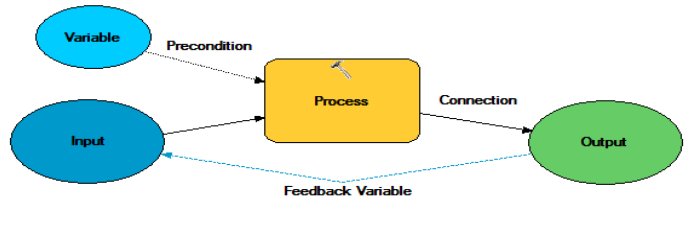
\includegraphics[width=\linewidth]{gfx/Methodology/old_project.png}}
\caption{An example model built in ArcGIS modelbuilder.}
\label{fig:inputs}
\end{figure}\\

The toolbox we created, comprised of ArcGIS functionalities with the core being the Cost Distance tool. The development was executed with the built-in Model Builder. Model Builder has the capability of invoking modules and algorithms through an easy-to-use Drag'N'Drop functionality. Although the preliminary model-development is significantly easier due to the GUI, applying more complex algorithms and connections between models and submodels, can quickly become unmanageable. 
The developed tool made it possible to simulate water advancing through the landscape, covering the parts of land that were below a certain predefined elevation, and connected to the source of the flood. \\

After completing that project, we were left wondering how this toolbox could be made available to an even greater amount of people. Another question that arose was how this tool could be made available freely without any of the software limitations that using a proprietary licensed software, like the ArcGIS software suite, provide.
In order to pursue such an endeavour, we must make sure that this new product has to offer at least the same functionalities as the one created before. In addition, the way it is developed has to provide us with greater distribution potential in order to ensure widespread availability to any interested organization or person. Keeping these ideas in mind, we reached the aforementioned problem statement and began working on this project.

\section{Workflow}
In order to be in accordance with the goals that we set, before working on the technical aspects of the project, we decided to split the project into several distinct phases. These phases comprise the general technical processes we would have to go through when completing the project. They are created in such a way that they divide our work into parts splitting the work into logical sub-parts. This division will also serve the purpose of making this report easier to read and more understandable.   
Each phase describes a different process of the project from setting up its foundations to the final, fully working prototype. \\
The phases will be described as being distinctive from each other. In reality this is not the case. Since this is a product of group work, it made a lot sense to divide the workload among the different members of the group. This would save a significant amount of time since not all different phases required more than one member working on that specific part. That being said, the way the work unfolded, it resulted in overlapping phases. This simultaneous development of parts of the application ensured that constant communication among the group members was a high priority, and also made sure that changes on existing and fundamental parts were not too time consuming. For example, tweaking of the PyWPS  in order to connect and enable specific functions as they get developed and deployed to the server, was a task that was worked on throughout the entire project.\\

Below, is a quick sketch of how the phases were planned to look:

\begin{description}
	\item [Start-up:]
This phase involves defining exactly what we wanted to attain with the project.

  \item[Phase 1 - Environment:] In this phase we performed the core setup of the project. To be more specific, we decided on which server our data and functionalities will be deployed upon. In addition, we decided on the software and the programming languages  we will use.
  
  \item[Phase 2 - Conversion:] In this phase we deal with the conversion of the already created model to a model that is compatible with the choices we made on the phase before. In fact, this part does not deal with anything other than that conversion. It is the core of the process because the vital processes of the service are developed here.
  
  \item[Phase 3 - Back-end:] In this phase, we create the foundation of the web service. To be more specific, it involves the back-end of our service. How it is structured in order to support all the functionalities that will be provided to the user. 
  
  \item[Phase 4 - Added functionalities:] All the added functionalities of the application are developed. This is where the extended functionalities of the service is developed, from creating a barrier to finding critical areas. 
  
  \item[Phase 5 - Front-end:]Here we mainly describe the front-end of the application. This is what the users sees and uses in order to get the results that they need. It includes all interactive parts of the web service that initialize various functions  that provide the user with results.

  \item[Writing:]As the project would become more and more finished, we will start writing. As mentioned we will keep notes, and write various parts that are important to memorize as the project progresses, but the writing will occur mostly when the project is fully finished. This is done because some aspects of the project might change during the course of the development, and we do not want to have to redo various written parts.
\end{description}

We expected the various phases to take up approximately three weeks but with five weeks set aside for Phase 4 where the functions were developed, a table of the estimated time for each phase is provided in \autoref{tab:phases}.\\

\begin{table}[h!]
\centering
\begin{tabular}{l | c | c | r}
Phase & From & To & Duration \\

Start-up & 02/02/15 & 16/02/2015 & 14 \\
Phase 1 & 16/02/2015 & 09/03/2015 & 21 \\
Phase 2 & 02/03/2015 & 23/03/2015 & 21 \\
Phase 3 & 16/03/2015 & 06/04/2015 & 21 \\
Phase 4 & 30/03/2015 & 04/05/2015 & 35 \\
Phase 5 & 27/04/2015 & 18/05/2015 & 21 \\
Writing & 11/05/2015 & 03/06/2015 & 23 \\
Finishing up & 03/06/2015 & 03/10/2015 & 7
\end{tabular} \\
\caption{Phases and their allotted time}
\label{tab:phases}
\end{table}\\

The phases of the project will be explained in detail on the next chapter. The way we will present the development of our work is aiming towards a more understandable and logically segmented report. That being said, we think that firstly presenting the completed phases and then documenting the other unsuccessful routes that we tried is, for us, the best way to communicate our work to the reader. To be more specific, the layout of the next section of the report will provide the reader with the process of creating a working prototype in detail. This means that the various tools and techniques that we use will be presented and explained along with arguments on why we think that this is the best available solution at the time of creation. After we are finished with documenting this part, we spend some time presenting the alternatives that we tested before reaching to that solution, if there are any, and provide the reasons and thoughts that lead us to abandon that specific course of action. By separating these two phases of development, we want to make sure that the reader can easily locate what they are looking for, i.e. suggested course of action or courses better avoided. 

\subsection{The practical foundation}
We decided to base the project, on a well-known location. This would make sure that the project would be grounded in reality, and make it easier to test the project consistently.
We decided on using Denmark as our reference country. This was first of all done, because the (previously mentioned) last project was based on working within Denmark as well, and this would give us a logical starting point for our model, and would provide a point of comparison for the results of the new application. 

Furthermore, the data standard for Denmark is very high. There are a variety of different DEMs that can be used, and they are created for a variety of purposes, as well as span a broad swathe of different resolutions. Additionally, they are free to use, and can be easily accessed from the Danish Geodata Agencies website {\href{http//:www.kortforsyningen.dk}{Kortforsyningen}}. 

Additionally, the landscape and weather in Denmark do not suffer from being very extreme. What this means is that the landscape as such is relatively uniform and does not experience sudden extreme highs or lows, and  the weather is also very consistent, and never experiences such extreme phenomena such as tsunamis. 

Some of the highest water levels ever recorded were between 4,3 meters (in Esbjerg) and around 5 meters (in Ribe around 1919). As mentioned, these were extremes, and the historical heights of floodings caused by storm water, have been in the area of 200 centimeters \citep{kyst}.

Towards the year 2050, DMI expects that there will be an increase in the water level between 10 and 50 centimeters in the internal areas of Denmark. \citep{dmi}

For this reason we decide to model floods in our application based on a water rise of 300 centimeters. The reason for this, is because it will reflect an “extreme” situation in Denmark, based on the heights provided by the historical records. Furthermore, it will also, to some degree, describe the expected water rise in Denmark.

\subsection{Calendar}
Each phase has a weeks overlap with the previous phase. This is done to indicate that as one phase is slowly finishing up, the next one will slowly start up. This also shows how dynamic the creation of a project such as this is. To give an overview of how we were expecting to progress with our project, we sketched the phases above into a so-called Gantt diagram. This gives a nice overview of this overlapping of the phases as mentioned above, and can be seen on \autoref{fig:gantt}.
\begin{figure}[h!]
\centering
\begin{ganttchart}[y unit title=0.4cm,
y unit chart=0.5cm,
vgrid,hgrid, 
title label anchor/.style={below=-1.6ex},
title left shift=.05,
title right shift=-.05,
title height=1,
bar/.style={fill=gray!50},
incomplete/.style={fill=white},
progress label text={},
bar height=0.7,
group right shift=0,
group top shift=.6,
group height=.3]{1}{20}
\gantttitle{Month}{20} \\
\gantttitle{February}{4} 
\gantttitle{March}{4} 
\gantttitle{April}{4} 
\gantttitle{May}{4} 
\gantttitle{June}{4}  \\

\ganttbar{Start-up}{1}{2} \\
\ganttbar{Phase 1}{3}{5} \\
\ganttbar{Phase 2}{5}{7} \\
\ganttbar{Phase 3}{7}{9} \\
\ganttbar{Phase 4}{9}{12} \\
\ganttbar{Phase 5}{12}{15} \\
\ganttbar{Writing}{15}{17} \\
\ganttbar{Finishing up}{17}{18} \\

\end{ganttchart}
\caption{Gantt-chart showing the overlap of phases}
\label{fig:gantt}
\end{figure}

%----------------------------------------------------------------------------------------
 % 
% Chapter 1

\chapter{Implementation} % Chapter title

\label{ch:theory} % For referencing the chapter elsewhere, use \autoref{ch:introduction} 

%----------------------------------------------------------------------------------------

As mentioned previously the work was divided into a series of phases. Before these commenced, we wanted to decide on which tools we were going to use for the application. 
We knew we wanted to make an online application that would enable a user to model the flooding of a provided area.  
To model the flood we decided on using GRASS at it is a powerful Open Source software, with a history being used in a variety of professional settings – such as the american army corps of engineers. Furthermore, the application allows easy access to it's core functions through a Python interface. 
GRASS is natively supported by the WPS called PyWPS. Therefore this seemed like a natural choice for our project. 
To gain the online application of the project, a web server would obviously be needed, and for this hosting of some sort, and we ended up using the Amazon Elastic Compute Cloud (or EC2) for this purpose.
The majority of the development was performed on machines running Ubuntu, so the syntax and explanations will therefore reflect this fact.
Now that we were set on the tools we were going to use, we were starting the actual implementation, we decided to sketch out how we expected the application would end up looking, and functioning.\\
\\

IMAGE OF THIS\\
\\

Now that we have a rough idea of how the project would be working, we could get started on implementing these ideas into an actual solution.

\section{Phase 1}
This phase involved setting up all the necessary preliminary settings, such as our local and server-side GRASS installations, the needed environment variables, and setting up a server. \\

\paragraph{Setting up a local scripting environment:} Instead of working directly on the server, and working with PyWPS we decided to create a local working environment using GRASS with Python, on our own machines. This was done to simplify the workflow and make sure that  we didn't have to update the server whenever changes were made to the code. \\
The syntax for running GRASS through Python and GRASS through the WPS differ, so it would have to be changed accordingly when porting it online, but this would allow us to get started immediately. \\
When working with GRASS, but not explicitly starting a GRASS session, a variety of environment variables have to be set. 

\begin{itemize}
\item \textsc{GISBASE}: This points to the top level directory of the GRASS installation
\item \textsc{GISDBASE}: GRASS' database location, usually initiated as grassdata.
\item \textsc{PATH}: The path location of GRASS, usually includes /script/ and /bin/.
\end{itemize} \\

These settings are set up in the header of the project, and for our set up look like this:

\begin{lstlisting}[language=Python]
gisbase = '/usr/lib/grass70'
os.environ['GISBASE'] = gisbase
os.environ['PATH'] += os.pathsep + os.path.join(gisbase, 'extrabin')
os.environ['GISDBASE'] = gisdb
\end{lstlisting}

When running the python script, it now initiates the GRASS environmental variables that are necessary for importing and using GRASS' functions.\\

\paragraph{Setting up the server:}Before being able to set up PyWPS, it is necessary to set up a server, capable of serving the processing service.  
As PyWPS was created with Linux in mind, and because the creators even specify that it works better on a Linux-based operating system, we wanted to make sure that the server was running this as well. Today there are a variety of different hosting services available, but for this project it was decided to use Amazon Web Services (AWS).\\

The main reason for running the server on this service is because several members of the group have had previous experience with launching minor applications on this platform, but also because it is possible to launch a so-called micro instance, which is free for the first year. The free-tier provides a very basic server, with little processing power and hard drive space – but for a proof-of-concept project such as this, it would suffice. \\
Initiating a server on Amazon's Elastic Compute Cloud (EC2) is easy, and only takes a couple of minutes. As several members of the group were already using the Linux-based operating system Ubuntu we decided to base the server this.\\
Connecting to your server is done using SSL, and when using Ubuntu, can be performed with the terminal. The only situation where this would not be so, is when having to upload specific files, for this a FTP client software is used.

\paragraph{Setting up Apache:}Every instance set up with Amazon, is provided with an IP address which can be used to visit the server using a browser. The Ubuntu image installed on the server did not contain a pre-installed web server, so it was necessary to install and configure this first.
Installing software on a machine running Linux is, and Ubuntu uses the package manager aptitude. Using the following terminal command, the web server is installed:

\begin{lstlisting}[language=Python]
sudo apt-get install apache2 
\end{lstlisting}

Now when visiting the IP address provided by Amazon, a standard Apache welcome-page greets the visitor.
The web server will serve the files that are placed in the following folder:

\begin{lstlisting}
/var/www/html/
\end{lstlisting}

So this is where most of our server-side changes would occur during the development of our application.\\

\paragraph{Installing GRASS:} The next step is setting up GRASS on the server. Version 6.4 was installed by using the following command:

\begin{lstlisting}
Sudo apt-get install grass
\end{lstlisting}

GRASS depends on a folder with the name grassdata on the computer's home directory. This functions as a database, and where it's input and output will be stored. Instead of setting this up from scratch, our local grassdata folders were copied straight to the server's home drive at

\begin{lstlisting} 
/home/ubuntu/
\end{lstlisting}\\

\textsc{\textit{Installing PyWPS}}\\

Now that Apache and GRASS have been installed, it was time to install the backbone of our entire project, PyWPS.
A thorough walkthrough of the installation of PyWPS can be found on our Github, so installation of PyWPS was performed into the folder of our webserver at the following directory:

\begin{lstlisting}
/var/www/html/pywps/
\end{lstlisting}\\

\subsection{Problems encountered}\\

\paragraph{Setting up GRASS scripting to run on a Windows machine:} It turned out that setting up the GRASS environment on a windows machine, was not very easy. This is because the GDAL and OGR bindings depend on a variety of specially created bindings when using them in a Windows environment, so this can cause trouble if you do not download the right ones.\\

\paragraph{Lack of documentation:} As the installation instructions of the PyWPS was not very well documented, and because a wide variety of settings have to be set correctly during installation, it was necessary to reinstall the server several times. This was both time consuming and frustrating, but the steps to install the service have now been documented greatly on our Github, so that hopefully someone else can now do it faster then we were possible at first. 

\paragraph{GRASS64 vs GRASS7:} We actually started by installing the newest version of GRASS, GRASS7. It turned out that there were some  incompatibility issues when using PyWPS with GRASS7. This meant that we had to downgrade the server-side GRASS package to GRASS64.\\

\section{Phase 2}
The model of this project is based on our previous project mentioned earlier. Since that project was developed in an ArcGIS environment, each functionality had to be converted to GRASS python modules. Some of the modules are not directly transferable between GRASS and ArcGIS, therefore we needed to find the best fitting functions that would also keep processing time at an acceptable level.\\

\begin{figure}[h!]
\centering
	{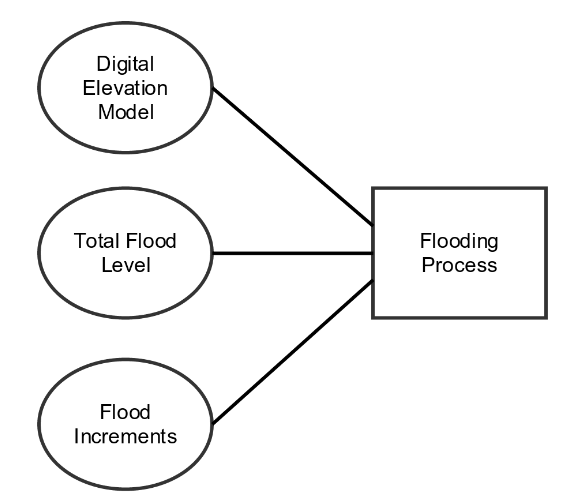
\includegraphics[width=.45\linewidth]{gfx/Phase_2/image.png}}
\caption{Inputs for the flooding model.}
\label{fig:inputs}
\end{figure}\\

As seen on \autoref{fig:inputs}, only one external data source is required, a DEM. According to the LOCATION used within GRASS, every imported DEM has to have a WGS 84 geographical projection. An important factor of the model, is that all web-mapping operations are done on Open Street Map, which uses a slight variant of WGS 84 as well. As is mentioned in theory, GRASS uses GDAL for importing several type of raster maps and OGR for importing vector datasets. Taking the advantage of these modules it is possible for the to use any raster, as long as it is project into WGS 84. Another input of the model is the maximum flood level and the water rise increments of flood. These numbers define the amount of loops necessary before the flooding is complete.\\
To flood the DEM, the model extracts those areas that are below current level of the iterator (and therefore flood). The first iteration will always be the sea level, where the actual flood level is 0. This extracts every cell with a value of zero. \\
This method will extract ALL areas that have a value of 0, which usually will generate several disconnected clumps of cells, located in different areas of the DEM. As our model has to generate a flood from one specific area (so as not to simulate that all streams and lakes in an area are filling with water) the model will require that the user interacts further. The user needs to choose from which source he/she would like flood the DEM from. The pre-selected point has a major role in this part of the model, as the flooding will be based on it. \\

After extracting every cell that is below the actual flood level, the process runs a cost distance analysis using the point as a source. The returned raster shows only one continuous area, for that level of the flood. The output cost raster is then converted to a vector with the value of the flood level. Each iteration extracts the land from the raster which is below the current flood level and select the continuous area depicting the actual flood on the land from the preselected source. 

The process is illustrated on \autoref{fig:continuous}. On \autoref{fig:allflood}, the algorithm identifies every possible cell that is under the current water level, indicated by the pink color. After the r.cost module has finished, the process returns a layer indicating which cells are reachable, as seen on \autoref{fig:actualflood}.\\

\begin{figure}[h!]
  \myfloatalign
  \subfloat[Every cell with a value less than the current flood level.]
  {\label{fig:allflood}  
  {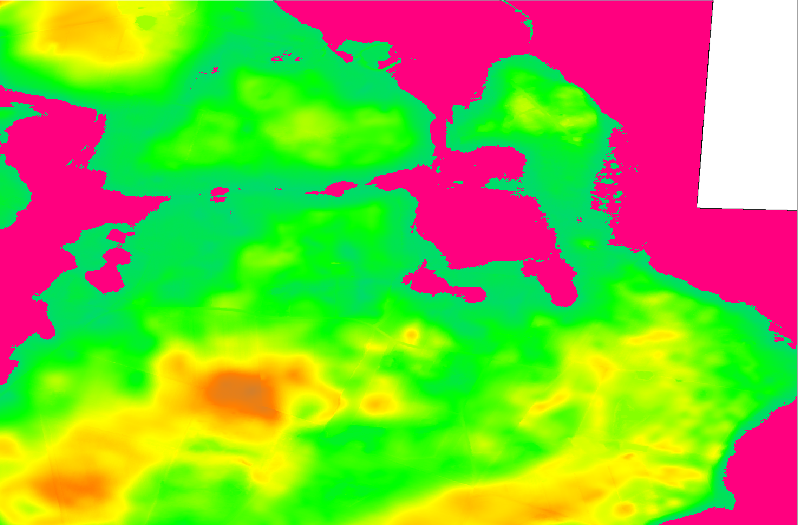
\includegraphics[width=.45\linewidth]{gfx/Phase_2/image2.png}}} \quad
  \subfloat[Cells reachable from the source point.]
  {\label{fig:actualflood}%
   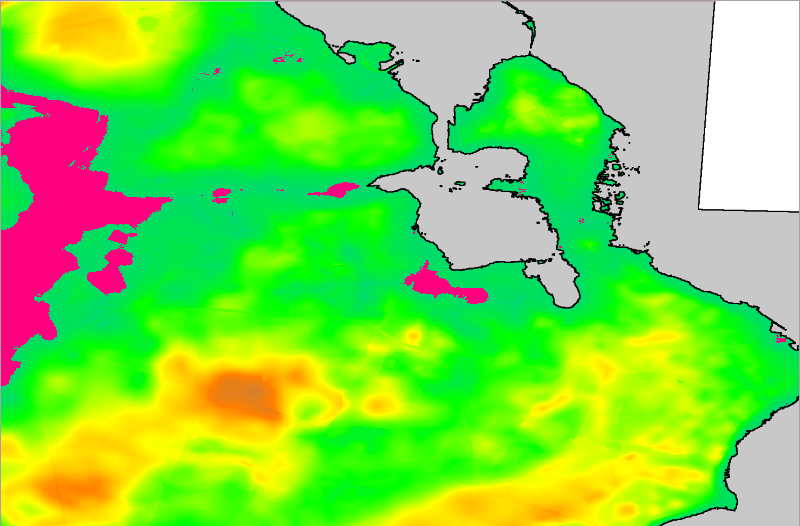
\includegraphics[width=.45\linewidth]{gfx/Phase_2/image3.png}} \\
 \caption{Figures indicating how r.cost is used to identify continuous areas}
 \label{fig:continuous}
\end{figure}

Every complex module from the earlier project has been taken out, and it has been simplified by using basic geoprocessing tools such as rasterizing, vectorizing, raster calculator and cost analysis. After the python - GRASS conversion was done, additional functionality was created, which will be discussed in \autoref{ch:phase4}.

\section{Phase 3}
This section will focus on the back-end of our web server. We begin by initializing Flask on our server. It is important to keep in mind that we earlier installed the Apache web server. After extensive research online, several different sources suggested a universal process on how to install Flask on an Apache 2 server. To go on, before actually installing Flask, we need to initialize mod\_wsgi. Mod\_wsgi is a tool that specializes in serving python applications from Apache servers. Installing mod\_wsgi is quite easy, and only takes a few lines of command line scripting (figure XXX).\\

\begin{lstlisting}
sudo apt-get install apache2 apache2-base apache2-mpm-prefork apache2-utils libexpat1 -ssl-cert
sudo apt-get install libapache2-mod-wsgi python-pip git
pip install flask
\end{lstlisting}\\

Following this installation we need to create an application.wsgi file. This is basically a file that contains code that initializes the application and comes with the .wsgi file extension. 
Now that Flask and prerequisites have been set up, it is time to look at what the backbone of the application looks like. At first, it is important to mention that the initial setup of the application will use Flask. To start with, and keeping in mind the way Flask actually works, we need a main Flask script that can initialize the application and connect various functions with its main core. In addition, that main script will also be connected to various html pages depending on where the user wants to navigate in our application.
The first action we took was to change the default path of our application in the server. Instead of using \textit{/var/www/html}, we started using \textit{/var/www/html/FlaskApp/FlaskApp}. This path will be referred to as the root url. After doing that, we create the script that will perform the functionalities of the application. That script is named \_\_init\_\_.py. Using Flask allows us to connect to various html scripts by using  only one main script. Depending on the URL of the page the user wants to get to, the corresponding HTML script is called and displayed on the user's screen. For example, as shown below (figure XXX), if the user visits our homepage, which is set by the \textit{\@app.route()}, then the \textit{'index.html'} will be initialized and displayed on his screen.\\

\begin{lstlisting}
@app.route('/')
def hello_world():
	return render_template('index.html')
\end{lstlisting}

The first action the user must perform in order to begin using the application is to upload a DEM. When the user clicks on the FLOOD button on our starting page, they get redirected to the root url/upload  section of the application. The way that section is working is that it expects a file to be posted. When that happens, it saves it to a pre-designated folder on the server. Right after that, we create a copy of the uploaded file and convert it from .tiff to .png. The reason behind that conversion is that we need to display the uploaded elevation model on a map for the user to see, which is vital to the next steps of the application. In order to be able to overlay an object on top of a map using leaflet, then that object has to be of .png or .jpeg format. All the aforementioned functions are included in the script below.\\

\begin{lstlisting}
def upload_file():

	if request.method == 'POST':
		file = request.files['datafile']
		if file:
			filename = secure_filename(file.filename)
			file.save(os.path.join(app.config['UPLOAD_FOLDER'], filename))
			src_ds = gdal.Open( os.path.join(app.config['UPLOAD_FOLDER'], filename) )
			formatimage = "PNG"
			driver = gdal.GetDriverByName( formatimage )
			fileName, fileExtension = os.path.splitext(filename)
			finalloca = '/var/www/html/FlaskApp/FlaskApp/static/images/' + str(fileName) + '.png'
			dst_ds = driver.CreateCopy( finalloca, src_ds, 0)
\end{lstlisting}

When the upload process is complete, a function is initialized allowing us to display that image on the map. Since we are using leaflet as a javascript library, in order to be able to display an image, we need to provide the function with the coordinates of the South-West and North-East corners of the image's display boundaries. To acquire this piece of information, we use gdal. The way we obtain the required coordinates are show below.\\

\begin{lstlisting}
			width = ds.RasterXSize
			height = ds.RasterYSize
			gt = ds.GetGeoTransform()
			minx = gt[0]
			miny = gt[3] + width*gt[4] +height*gt[5]
			maxx = gt[0] + width*gt[1] + height*gt[2]
			maxy = gt[3]

			return redirect(url_for('upload_file',filename=filename,minx=minx,miny=miny,maxx=maxx,maxy=maxy))
\end{lstlisting}\\

The final step we need to take before we are able to show the uploaded image, is to pass coordinates back to the html document that is responsible for showing that image so that a javascript function can get and display the image properly. That is achieved by the final line of the script on the image above.

\subsection{Problems encountered}
Having presented a viable option on how our web-service is structured and what tools we used to achieve successful functionalities, it is time to examine what other alternatives we have explored that did not result in acceptable results.\\
As presented above, we use Flask to create the back-end of our application. This decision was not our initial one, since none of the group members  had any particular experience using this framework. That being said, it normally would seem a rather unorthodox approach to start using a tool that no one is familiar with at the middle of our project development, since that is when we introduced Flask to the project. The truth is that our first option was to use an HTML and JavaScript core and PHP to upload the user provided input to the application. To be more specific, we would have an HTML document that allowed the user to upload a file and use PHP to convert that file from .tiff to .png. Then that PHP script would call a python script that calculated the bounding box coordinates of the image and then pass them on to a second HTML document, to be used by a JavaScript function that overlays the image on the map. The reason we considered using that approach is that we were more accustomed to using PHP to perform specific functions such as manipulating and uploading a file. On the other hand, this approach is clearly much more complicated than the one we finally used. Especially, if we keep in mind on how many different programming languages are included in that approach and how many different scripts we need to connect in order for it to work.  In addition, the transition from PHP to python was never achieved up to the point where we decided to change directions.\\

What we managed by using Flask instead, was to exclude the use of PHP and thus reduce the complexity of the script by a great deal. Firstly because we do not have to worry about creating extra connections with various other scripts. In fact Flask, and the way it is designed to operate, simplified our development considerably. It allowed to have a central script of python that inherently interconnected with all our HTML scripts and supported other python functions at the same time.

\section{Phase 4}
\label{ch:phase4}

To expand on the functionality of the application, we have additional functionalities and tools, which could be a tool used for flood or disaster management. 

\subsection{Identifying critical areas}
\subsubsection{Outlet analysis}
During the development of the pour-point analysis, we encountered sine problems. At the beginning, we tried to derive this problem from a watershed analysis, based on the identification of watershed's outlet. Our hypothesis was , that the flood  would flow backwards through the flow accumulation and flow stream model to the source cells and when the water enters through an outlet, to a new watershed, than that area would become flooded. Therefore we created a workflow which extracts only the outlet of the watershed. As it presented in the theory part, we used the watershed(r.watershed) and flow accumulation module (r.terraflow) in order to determine the inlet-outlet location of the watershed. We tried to establish an algorithm for relative watershed determination based on the investigated DEM. We set up, the minimum threshold size of a watershed, has to be at least the ten percent of the DEM. After the workflow run the previously used neighborhood analysis(r.neighbor) with diversity method with we could extract the watershed borders on a raster. Using the terraflow module with single flow direction setup, we created the a flow accumulation raster. This is important to determine the inlet/outlet location. Using the single flow direction method, every outlets will be located on the border of a watershed where the flow accumulation is the maximum. With this approach we though we got can a relatively good result to determine where the flood flow will enter to new area, however the testing of the algorithm showed its failure of our planned purpose.

\subsubsection{Pour point analysis}
Only providing the a extent is not enough when wanting to prepare against the impact a disaster. We wanted to provide more information about the flood regarding areas that might be particularly dangerous. After monitoring the  spread of the flood using our simple model, we realized there were areas where a relatively large area got flooded immediately. This can occur when the flood steps over a natural barrier, with a lower elevation than the surrounding area. This is what we call a “pour-point”. One of our major challenge was how to identify this behaviour and to locate the actual position of these critical points automatically.// 
Since these pour point phenomena are very dependent how the process is run; which increment the water is rising in; which output (raster or vector) are we working with. Firstly, we realized that to give an accurate flooding the increments would have to with 1 cm water increments. By using this increment, this flood can be accurate enough to identify major changes between consecutive flood levels.

\begin{figure}[h!]
\centering
	{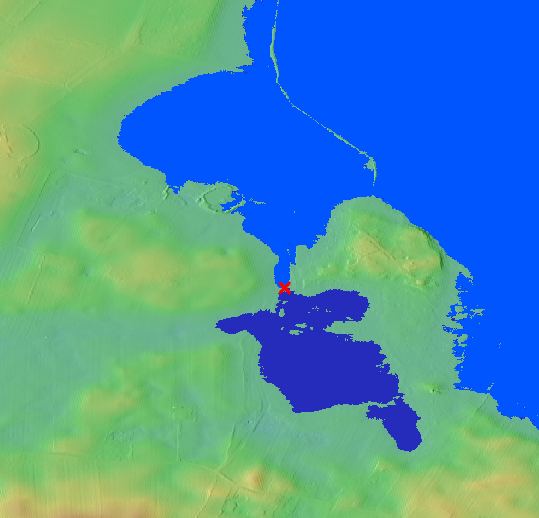
\includegraphics[width=.45\linewidth]{gfx/Pourpoint.png}}
\caption{Figure showing the pourpoint we are trying to identify.}
\label{fig:pourpoint}
\end{figure}

\autoref{fig:pourpoint} shows two consecutive flood extents with 140cm(light blue) and 141 cm (dark blue) water rise. The red area indicated on the figure is what we needed to locate. Although it might seem to be a fairly easy procedure, we have to add that the large blue area on the image is not the only area that has increased in size between the two stage of flooding. Along the border of 140 cm (light blue) flood level, there are a relatively small areas or cells  which are flooded at the 141 cm. In order to avoid small or irrelevant pour point identification the following workflow was created. 
As described in phase 2, after each flood extent the output is stored in both raster and vector format. In order to overcome the situation to identify pour points at each level, we implemented a condition which checks the size difference between each consecutive stage. We added an area field for each flood extent polygon, thereby we can built a decision analysis based on the flooded area. If the difference between two consecutive flood stages is larger than one percent of the investigated DEM, then the pour-point analysis workflow is triggered. The two investigated flood extents are subracted from each other, a selection based on its area field is conducted. By performing this subtraction, a lot of polygons are created. For each polygon the process calculates an area field and selects only those that are larger than 1000 square meters. This criteria is to avoid relatively small areas (indicated in grey on \autoref{fig:twofloods}, which the pour point analysis would not make a reasonable investigation since their size is negligible compared to those area which have a larger impact on the advancing of the flood (indicated by the red color) . After the exclusion, only those areas which have a larger extent than the previously mentioned criteria are left.\\

\begin{figure}[h!]
  \myfloatalign
  \subfloat[Showing two flood extents.]
  {\label{fig:twofloods}
  {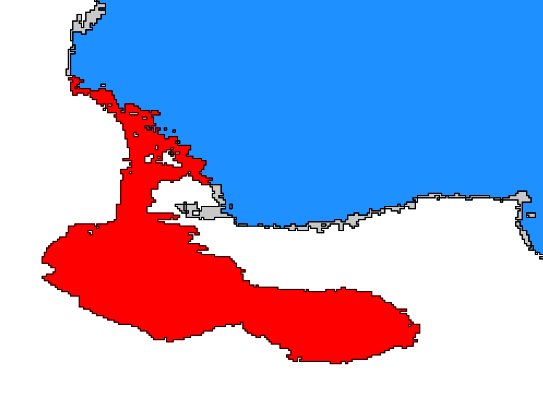
\includegraphics[width=.45\linewidth]{gfx/Phase_4/Pourpoint2.png}}} \quad
  \subfloat[Showing line of pour points.]
  {\label{fig:allthepoints}
   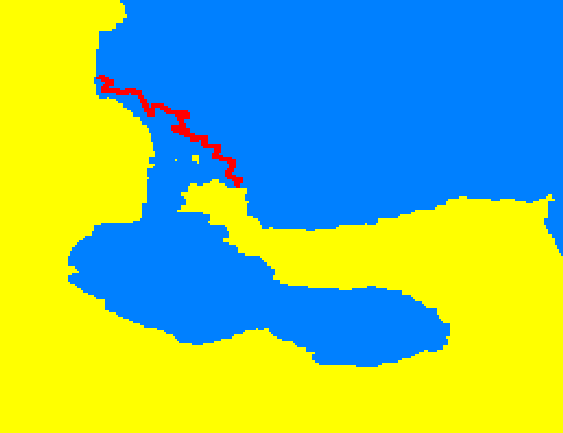
\includegraphics[width=.45\linewidth]{gfx/Phase_4/Pourpoint3.png}} \\
  \caption{Showing the concepts of finding the pourpoints.}
  \label{fig:pourpoints}
\end{figure}

The remaining polygon(s) are converted back to raster and merged with the previous raster extent of the flood, thereby a new raster map represents, the previous flood (blue) and the actual flood (red) with increments which are over the criteria. This raster has raster values where the flood extent exists and NULL values everywhere else.
Afterwards a neighborhood analysis (r.neighbors) is conducted, based on the diversity method – which is based on the Moore-Neighborhood. This method is applied in order to find the location, where the raster changes values, since that place is where the flood enters into the new area. In \autoref{fig:twofloods} a black border can be seen, where the red and blue area touch. The process need to identify automatically only that border which connects the two different flood stage in the critical location – I.e the pour points. The diversity method can be used to identify only the border cells as it seen in \autoref{fig:allthepoints}.
After the identifying the pour-point cells with the above-mentioned analysis, the algorithm then extracts those cells and converts them to vector points. \\

To have the pour-points as vector points is partly because we can then easily store information about the necessary height of a barrier at this place, and so that they easily can be displayed and manipulated on our web map following the analysis procedure. 
For the better understanding and providing essential information of the critical area, we decided to add th elevetion of the pour-point location and the maximum flood depth based on the actual scenario. This was done by point sampling method of GRASS. (r.what.rast). Sampling method extracts those cell attribute, where the vector points act as a centroid of the cell square. \\

\subsection{Barrier placement}
An integral part of the application is allowing the user to implement barriers that will mitigate the effects of the flood. The user will be able to determine whether an area can be secured by the implementation of obstacles in the landscape or how the flood can be affected by installing a barrier in a given position. \\
The general operation of having the barrier placement process available to the user starts after the flood simulation has been performed and completed. This is because the user has to have an overview of the overall situation of the flood and the location of the critical areas in the landscape, before starting placing barriers in random areas and in an arbitrary fashion. We believe that this would ensure that the entire process of finding a suitable solution to a flood situation is fast since performing the advanced simulation can take a lot of time.\\

The process begins by getting the input from the webpage where the user draws a barrier on a web map. This results into the creation of a GeoJSON file that is then transferred to the python function that creates the does the modelling. Since the barrier is in GeoJSON format, we need to convert it to raster in order to hardcode it into the elevation model. Normally, converting the barrier to raster and then adding it to the elevation model would be enough. Unfortunately, we stumbled upon a quite unexpected problem. The sections of the barrier that are not completely vertical or horizontal are rasterized in an erroneous fashion. To be more specific, in these sections the cells are not connected with a shared side of cell. Instead, they are connected by sharing an edge. The figure below demonstrates the problem when the barrier is converted to raster, as can be seen in \autoref{fig:rasterize}.\\

\begin{figure}[h!]
  \myfloatalign
  \subfloat[Rasterized barrier.]
  {\label{fig:rasterize}
  
\includegraphics[width=.45\linewidth]{gfx/Phase_4/Barrier1.png}} \quad
  \subfloat[Problem areas.]
  {\label{fig:problemareas}%
   
\includegraphics[width=.45\linewidth]{gfx/Phase_4/Barrier2.png}} \\
  \subfloat[Generating pixels in the designated areas.]
  {\label{fig:barrier3}
  
\includegraphics[width=.45\linewidth]{gfx/Phase_4/Barrier3.png}} \quad
  \subfloat[Fixed barrier.]
  {\label{fig:barrier4}
  
\includegraphics[width=.45\linewidth]{gfx/Phase_4/Barrier4.png}}
  \caption[Generated extra pixels]{The process of fixing the rasterized barrier.}\label{fig:barriers}
\end{figure}

The problem depicted above is quite unexpected especially if we take note of that fact that the conversion ignores several cells that intersect with the barrier line and instead keeps only cells that are connected diagonally with each other. That leads to gaps on the barriers that would allow water to flow through them. In order to deal with that problem we have developed the following solution. \\
Practically, we need to assign the pre-designated value of the barrier height to one of the cells per diagonal intersection to create a continuous raster of the barrier, as indicated on \autoref{fig:problemareas}. 

In order to do that, first we extract the edges of the non-vertical, non-horizontal sections of the barrier. In addition, we extend those cells by one cell in the northerly direction. That action is performed by the following part of the script, as seen on \autoref{fig:barrier3}.

\begin{lstlisting}

\end{lstlisting}

As can be noted in the script above, we are using neighborhoods in order to extract the necessary cells. In fact, we are not using full neighborhoods (e.g. Moore Neighborhood) but specific cells that exist in the neighborhood of the cell mapcalc is actually querying. In order to query the correct cells, we are required to know their relative coordinates to the center cell that is queried. These relatives coordinates are displayed on \autoref{tab:relcoord}.\\

\begin{table}
\centering
\begin{tabular}{l | c | r}
-1,-1 & -1,0 & -1,1 \\
\hline \\
0,-1 & 0,0 & 0,1 \\
\hline \\
1,-1 & 1,0 & 1,1 \\
\end{tabular}
\caption{Relative cell coordinates to the center cell (0,0)}
\label{tab:relcoord}
\end{table}\\

The result of this edge selection is shown on the figure below (figure XXX).\\
\\


Since we have the edges of the barrier, we go on by expanding each one by one cell, as mentioned above, and merge the resulting raster with the initial barrier raster. That is done with the following script:\\

\begin{lstlisting}
gscript.run_command('r.patch', inputs=['edges_1_1_ext','edges_11_ext','barr_raster'],output='merged)
\end{lstlisting}\\

The final step in order to complete the barrier correction and deployment to the landscape is to hardcode it to the elevation model. Which is done with the following script: \\

\begin{lstlisting}
gscript.run_command('r.mapcalc', expression='original_b = if(isnull(merged),original,original+merged)')
\end{lstlisting}

This process results in the elevation model shown on \autoref{fig:fixedbarrier}.

\begin{figure}[h!]
\centering
	{
\includegraphics[width=0.75\linewidth]{gfx/Phase_4/Barrier5.png}}
\caption{Figure showing important concepts when working with watersheds}
\label{fig:fixedbarrier}
\end{figure}

By observing the result above, someone might think that it is difficult to observe the actual barrier and distinguish it from the elevation model. Unfortunately, this is the result of merging the two rasters together. It is logical that the results are not visually distinctive since they are in fact one raster represented by a sliding color scale.

\subsection{Problems encountered}
The main issue with the process of creating the barrier and performing the necessary correction was the necessity of actually performing the correction of it. That means that normally, the conversion of a linear vector file to raster should not behave the way we described above. we assumed that GIS software suits, such as QGIS and GRASS as well as ArcGIS, address issues as connectivity of cells in identical fashion. But unfortunately that was not the case. In fact, ArcGIS considers cells that share an edge (diagonal connection) as connecting cells and will include them in a raster to vector conversion. On the other hand, QGIS and GRASS does not. This lead us to dedicate a considerable amount of time in creating a solution.\\

Another issue that we faced was the lack of documentation on the mapcalc function that we used in this process. Despite following the existing documentation closely, we ran into problems that should not have existed. Initially, the proposed solution to the barrier problem consisted of a much more compact script that performed a universal query on all the cells of the barrier raster in order to cover its gaps. Unfortunately, for reasons yet undiscovered, that solution did not produce any results. The script we used can be seen below at its final state before we decided to develop the solution that performed as expected.

\begin{lstlisting}
corr_barrier = if(isnull(barr_raster), if(barr_raster[0,-1] == 3 && (barr_raster[-1,0] == 3 || barr_raster[1,0] == 3) , barr_raster, null()) || if(barr_raster[0,1] == 3 &&  (barr_raster[-1,0] == 3 || barr_raster[1,0] == 3), barr_raster, null()), barr_raster)
\end{lstlisting}

\section{Phase 5}
This phase involves setting up the necessary website relevant elements. This means both HTML, Javascript, web mapping and the understanding of PyWPS.\\

\paragraph{PyWPS:} As the the main functionality of our script was developed, we began porting the script to PyWPS syntax. 

The output cannot be defined dynamically. 

As mentioned in the theory part, every PyWPS must include 
\begin{itemize}
\item \_\_init\_\_ 
\end{itemize}
and 
\begin{itemize}
\item execute.
\end{itemize}
  
The various settings we set up to be:

\begin{itemize}
\item identifier = "flooding",
\item title = "Flooding",
\item abstract = "This process is used to flood a DEM with water",
\item version = "1.0",
\item grassLocation = "/home/ubuntu/grassdata/WGS\_1984",
\item statusSupported = True,
\item storeSupported = True
\end{itemize}

The most un-intuitive of these settings are the \textit{grassLocation}, \textit{statusSupported} and \textit{storeSupported}. 
We set \textit{grassLocation} to our predefined database folder. This is done in order to make sure that the uploaded data will work within a coordinate system, and that we can do the proper calculations on it.
When setting \textit{statusSupported} to True, means that the process can run asynchronously. 
And finally, using \textit{storeSupported} means that it is possible to deploy the results to the server, for later usage. 
After this has been set, we define the needed inputs. As mentioned previously, we want the user to provide a DEM and a point indicating where the flooding should occur from. Therefore we must inform the program that we will be expecting an image and a GeoJSON file. 

\begin{lstlisting}
self.rasterin=self.addComplexInput(identifier='rasterin',
		   title="input image",
	   	   formats = [{'mimeType': 'image/tiff'}, {'mimeType': 			             	'image/geotiff'}, 	   {'mimeType': 'application/geotiff'}, 		            {'mimeType': 'application/x-	   geotiff'}])
	   	   
self.vectorin = self.addComplexInput(identifier="vectorin",
		     title="Input point",
		     formats = [{"mimeType":"text/json","encoding":"utf-			              8","schema":None}])

\end{lstlisting}

After having defined the inputs. It's is also necessary to define the outputs. We want to provide the user with a raster of the flooding and the extent of the flooding as a vector file. Furthermore, after the process has completed, we want to provide an in-browser image of how the actual flooding looks. Because very few browsers natively support the display of TIFF images, we will output a JPEG as well:\\


\begin{lstlisting}
self.outputImage0=self.addComplexOutput(identifier="output0",title="output image", asReference=True)

self.outputImage1=self.addComplexOutput(identifier="output1",title="output image", asReference=True)

self.outputVector=self.addComplexOutput(identifier="output2",title="output vector", asReference=True)

\end{lstlisting}

By setting the setting \textit{asReference} to True, the output will not be delivered straight back to the user, but will be provided as a link to the location in which it is stored on the server. When returning images with PyWPS they get delivered as Base64 images, which means that they are returned as a long string of text. This can reduce the loading times significantly, and can for very large images also freeze the computer handling them. Furthermore it has the advantage, that if a user should lose connection, the images can still be recovered. 

Now that the initialization settings have been defined, the execute method can be set up. In general the code looks very similar to the functions created earlier, so they will not be explained here further (and they can be found on the previously mentioned GitHub page). 
After creating the service, they are placed in the processes folder on the server. Furthermore the \_\_init\_\_.py file is updated to now include the uploaded file. 
After having set up the script in PyWPS, and transferring them to the server, they are reday to be called. This can be done through the web browser.
In general it is possible to call either a GetCapabilities, Execute or DescribeProcess. For this project it will only be necessary to Execute a process, as this project is not meant to be accessed outside of our webapplication interface. 
They way the WPS service is requested from the server, I.e a flooding service with the identifier “flooding”, is called like follows:

\begin{itemize}
\item http://52.17.144.192/cgi-bin/pywps.cgi?request=execute&service=WPS&version=1.0.0&identifier=flooding&datainputs=[rasterin=<LINK TO DEM>;vectorin=<GEOJSON AS STRING>]
\end{itemize}

The server will process the request, and return a XML document with links to where the outputs of the process are stored. 

\paragraph{Setting up the design:} Using the power of Flask as much as possible, we wanted to make the website have as small of a footprint as possible. 
The application would consist of a welcome page with a brief introduction which would link the user to the “actual” application, which would be followed by a multi-layered page, that would guide the user through the process of flooding. 
IMAGE OF FRONTPAGE → IMAGE OF UPLOAD
Using the free Twitter Bootstrap CSS theme, it is possible to quickly create some working HTML pages. 

As the front page mostly contains information about the projects capabilities, this part will mostly focus on the second page. 

To guide the user through the process of flooding, it was decided to split the entire process into three steps:
\begin{itemize}
\item Step 1: Upload DEM
\item Step 2: Select Ocean
\item Step 3: Get Results
\end{itemize}
The three steps consist of various HTML parts that are hidden from the start, and as the user clicks through the steps, the next one is shown and the previous one is hidden. This is done using the following jQuery commands:

\begin{lstlisting}
$.(#step1).hide();

$.(#step2).show();
\end{lstlisting}

At most of the stages, asynchronous requests or operations will be performed. As they can take some time, we want to give the user some feedback that the page is loading. This is done by creating an overlay that takes up the entire screen, and includes a loading icon. The icon is hidden, but gets shown when a request is performed, in the same manner as above.
To describe how the outlined stages work we will go through them below. 

\textsc{Step 1 – Upload DEM:}
In this step the user uploads a DEM. Most of the functionality here is dependant on the functionality of Flask. So the only thing necessary to add here, is a HTML form with the capability of letting the user browse his computer for a DEM, and then clicking a button to upload it. 

\textsc{Step 2 – Select Ocean:}
In this step we want the user to select from where the flooding will occur. 

This entails showing the uploaded image on a webmap, making the user able to place a marker on the map, and then sending this information to the server.

When the upload has completed, the page refreshes. This means that the page clears all set variables. This is an issue when wanting to stay on the same page, but to load a different step. As Flask adds a variety of variables to the URL of the page, a workaround for this problem is to check to see if the URL contains  one  of the variables assigned by the Flask upload script:

\begin{lstlisting}
url = window.location.href;

if (url.indexOf("filename") > -1); {
	STEP 2

\end{lstlisting}

As mentioned, we want the DEM to be uploaded to a webmap. To do this a copy of the uploaded is created as a JPEG, which then can be used to overlay on the map. The JPEG cannot contain embedded coordinates. Using Flask, the corners of the uploaded TIF are extracted, and get returned to the URL of the webpage.
The format of this is something like:

\begin{itemize}
\item http://52.17.144.192/upload?minx=COORD&miny=COORD&maxx=COORD&maxy=COORD&filename=FILENAME
\end{itemize}

To extract the relevant data the following JavaScript code is executed:

\begin{lstlisting}
var findcorners = url.replace("http://52.17.144.192/upload?");
var findcorners2 = findcorners.split("&")
var filename = findcorners2[4].split("=")
var coordinatesforuse = [];
var expendable;
for (var i = 0; i < findcorners2.length; i++) {
    expendable = findcorners2[i].split("=")
    coordinatesforuse[i] = expendable[1];}
These are then stored into variables with a readable format:
var south = coordinatesforuse[0];
var west = coordinatesforuse[1];
var north = coordinatesforuse[2];
var east = coordinatesforuse[3];

\end{lstlisting}

Lastly they are prepared for insertion as the bounding box for the uploaded image, into the leaflet map:


\begin{lstlisting}
imageBounds = L.latLngBounds([
      [west, south], // Southwest
      [east, north] // Northeast
]);
\end{lstlisting}

As the uploaded TIF is converted into a PNG, but not returned to the URL, we are manually going to setup the URL where the PNG version of the uploaded image can be found:

\begin{lstlisting}
var imageuse = filename[1];
var imageaspng = imageuse.replace(/\.[^/.]+$/, ".png")
var variable = 'static/images/' + imageaspng;
var imageUrl = variable;
\end{lstlisting}

Now that all of this is done, we can initiate our map. Add the uploaded PNG as an overlay to our MapBox image, and define the marker that will be used.   

\begin{lstlisting}
// Initiate map "around" the uploaded DEM
var map = L.mapbox.map('map', 'piratosthegreat.i7aeacaf').fitBounds(
imageBounds);
// Add the DEM to the map
var overlay = L.imageOverlay(variable, imageBounds).addTo(map);
// Define marker
var marker = L.marker([16.436673, 38.322712], {
		icon: L.mapbox.marker.icon({
		'marker-color': '#f86767'
    })
});
\end{lstlisting}

To make it easier to find the ocean underneath the overlaid image, a transparency slider is added. This slider is provided by MapBox and can be freely found in their documentation.

The final thing is to add the onClick functionality of adding a point when clicking on the map, and to be able to send it to the server as a GeoJSON. This was done as follows:


\begin{lstlisting}
   map.on('click', function(e) {
               marker.setLatLng(e.latlng).addTo(map);

               markercoords = marker.getLatLng()

               geoj = [{
                   "type": "FeatureCollection",
                   "features": [{
                       "type": "Feature",
                       "properties": {},
                       "geometry": {
                           "type": "Point",
                           "coordinates": [markercoords.lng,
                             markercoords.lat
                           ]
                       }
                   }]
               }];
           });
\end{lstlisting}

We decided to add the possiblity for the user to choose between two different types of flooding at this stage. Either to do a quick flooding simulation, or a more advanced flood.
As soon as the relevant button is clicked, an asynchronous request is sent to the relevant PyWPS service.

\textsc{Step 3 – Get Results:}
Because of the response document from the PyWPS service being the same for either call, the structure and functionality of the asynchronous request performed will be (mostly) the same for both requests. So therefore only one request will be described here. 
The buttons used to send the request have been marked with either a advancedflood or simpleflood ID. In this instance we wil look at the advanced flood async request.
We have stored the relevant PyWPS URL in a variable in our script, and we have replaced relevant input with the data uploaded by the user 

\begin{lstlisting}
var preconpath = 'http://52.17.144.192/cgi-bin/pywps.cgi?request=execute&service=WPS&version=1.0.0&identifier=flooding&datainputs=[rasterin=http://52.17.144.192/static/images/' + imageuse + ';vectorin=' + JSON.stringify(geoj[0]) + ']';
\end{lstlisting}

The request we will perform is a standard jQuery async request to the PyWPS by using \textit{\$.get()}. This is encased in a when and a done function as follows: \textit{\$.when(\$.get()).done();}

This sets the script up in such a way that, when the asynch request is done, it launches some other code. 
The when and async request code looks like the following:

\begin{lstlisting}
$.when(
$.get(xmlPath, function(xml) {
        $("#overlay").hide();
        $(".step2").hide();
        $(".step3").show();
// Find the elements in the response XMl that contain our data
        $("wps\\:ProcessOutputs", xml).find("wps\\:Reference")
         .each(function(i, value) {
                  var imagepath = value.getAttribute("href");
                   var imagepathbroken = imagepath.split("/");
                  outputimagearray.push(imagepathbroken[5])
});
}, 'xml')
)
\end{lstlisting}

What this does is to get the XML document returned from PyWPS, traverse it and for each result, store it in a variable called outputimagearray.
When this is done it takes the outputs stored in the above mentioned array, and adds them to the website as an overlay to a map, and with possibility of downloading them.

\begin{lstlisting}
.done( function() {
               $(".loading").append('<div class="map" id="map1" style="height: 		500px; width: 100%;">')
               var map = L.mapbox.map('map1', 'piratosthegreat.i7aeacaf')
               .fitBounds(imageBounds);

               var outputimagesimple = 'static/outputs/' + outputimagearray[1];

               var overlay = L.imageOverlay(outputimagesimple, 				imageBounds).addTo(map);

               overlay.setOpacity(1.0);

              var featureLayer = L.mapbox.featureLayer()
              .loadURL('/static/outputs/' + outputimagearray[0])
              .addTo(map);

               $(".loading").append('<form method="get" action="http://52.17.144.192/static/outputs/' + outputimagearray[2] + '"><button class="btn btn-success btn-lg btn-block" type="submit">Download data !</button></form>')
             });
});
\end{lstlisting}

\subsection{Problems encountered}
\paragraph{Currently does not work on Chrome:} The way the URL's are formed, with variables added to them, do not work well with Chrome- This is an issue that can probably easily be fixed, but during this process there was not time to discover how to solve this issue. 

\paragraph{It is not possible to overlay a TIF:}
It is not possible to overlay a TIF onto the Webmap, and as such we had to also create a copy of the uploaded file, as a PNG. This does not take a long time, but makes it more tricky to make the entire process work the way we intend it to.  

\paragraph{At the moment flooding can only occur from one place:}
The way the GeoJSON creation is set up, and the way that the marker gets added to the map, the flooding can only occur from one spot. This should be relatively easily remedied, but at the time of creation, it was deemed satisfactory that the flood could only occur from one location.

% Chapter 1

\chapter{Analysis} % Chapter title

\label{ch:introduction} % For referencing the chapter elsewhere, use \autoref{ch:introduction} 

%----------------------------------------------------------------------------------------

 % Chapter 3
% Chapter 1

\chapter{Discussion} % Chapter title

\label{ch:introduction} % For referencing the chapter elsewhere, use \autoref{ch:introduction} 

%----------------------------------------------------------------------------------------

 % 
%% Chapter X

\chapter{Chapter Title} % Chapter title

\label{ch:name} % For referencing the chapter elsewhere, use \autoref{ch:name} 

%----------------------------------------------------------------------------------------

\section{Section Title}

Content

%------------------------------------------------

\subsection{Subsection Title}

Content

%------------------------------------------------

\subsection{Subsection Title}

Content

%----------------------------------------------------------------------------------------

\section{Section Title}

Content % Chapter 4 - empty template

%----------------------------------------------------------------------------------------
%	THESIS CONTENT - APPENDICES
%----------------------------------------------------------------------------------------

\appendix

\part{Appendix} % New part of the thesis for the appendix

% Appendix A

\chapter{Appendix Test}

%----------------------------------------------------------------------------------------

\lipsum[13-14]

%----------------------------------------------------------------------------------------

\section{Appendix Section Test}
\lipsum[15]

\graffito{More dummy text}
\lipsum[16]

%----------------------------------------------------------------------------------------

\section{Another Appendix Section Test}
\lipsum[17]

\begin{table}
\myfloatalign
\begin{tabularx}{\textwidth}{Xll} \toprule
\tableheadline{labitur bonorum pri no} & \tableheadline{que vista}
& \tableheadline{human} \\ \midrule
fastidii ea ius & germano &  demonstratea \\
suscipit instructior & titulo & personas \\
\midrule
quaestio philosophia & facto & demonstrated \\
\bottomrule
\end{tabularx}
\caption[Autem usu id]{Autem usu id.}
\label{tab:moreexample}
\end{table}

\lipsum[18]

\begin{lstlisting}[float,caption=A floating example]
for i:=maxint to 0 do
begin
{ do nothing }
end;
\end{lstlisting} % Appendix A
%% Appendix X

\chapter{Appendix Title}

%----------------------------------------------------------------------------------------

% Content begins here % Appendix B - empty template

%----------------------------------------------------------------------------------------
%	POST-CONTENT THESIS PAGES
%----------------------------------------------------------------------------------------

\cleardoublepage% Bibliography

\label{app:bibliography} % Reference the bibliography elsewhere with \autoref{app:bibliography}

\manualmark
\markboth{\spacedlowsmallcaps{\bibname}}{\spacedlowsmallcaps{\bibname}} 
\refstepcounter{dummy}

\addtocontents{toc}{\protect\vspace{\beforebibskip}} % Place the bibliography slightly below the rest of the document content in the table of contents
\addcontentsline{toc}{chapter}{\tocEntry{\bibname}}

\bibliographystyle{plainnat}

\bibliography{Bibliography} % Bibliography

\cleardoublepage% Colophon (a brief description of publication or production notes relevant to the edition)

\pagestyle{empty}

\hfill

\vfill

\pdfbookmark[0]{Colophon}{colophon}

\section*{Colophon}

This document was typeset using the typographical look-and-feel \texttt{classicthesis} developed by Andr\'e Miede. The style was inspired by Robert Bringhurst's seminal book on typography ``\emph{The Elements of Typographic Style}''. \texttt{classicthesis} is available for both \LaTeX\ and \mLyX: 

\begin{center}
\url{http://code.google.com/p/classicthesis/}
\end{center}

\noindent Happy users of \texttt{classicthesis} usually send a real postcard to the author, a collection of postcards received so far is featured here: 

\begin{center}
\url{http://postcards.miede.de/}
\end{center}
 
\bigskip

\noindent\finalVersionString % Colophon

\cleardoublepage% Declaration

\refstepcounter{dummy}
\pdfbookmark[0]{Declaration}{declaration} % Bookmark name visible in a PDF viewer

\chapter*{Declaration} % Declaration section text

\thispagestyle{empty}

Put your declaration here.
\bigskip
 
\noindent\textit{\myLocation, \myTime}

\smallskip

\begin{flushright}
\begin{tabular}{m{5cm}}
\\ \hline
\centering\GiannisName,\DavidName and \EmilName \today \\
\end{tabular}
\end{flushright}
 % Declaration

%----------------------------------------------------------------------------------------

\end{document}
